\documentclass[twocolumn]{aastex62}
%Following line instructs TeXShop to use latex + ghostscript:
%!TEX TS-program = latex
%\documentclass[12pt]{article}
%\documentclass{/Users/adam/papers/latexfiles/emulateapj}
%\documentclass{/Users/adam/papers/latexfiles/emulateapj}
%\usepackage{/Users/adam/papers/latexfiles/emulateapj5}
%\usepackage{/Users/adam/papers/latexfiles/deluxetable}

%\special{! /pdfmark 
%            [/View [/XYZ null null 1]  % unspecified x and y offset, 100% zoom
%             /Page 1
%             /PageModehttps://www.sharelatex.com/4759396695vhbmwsvkbydp /UseThumbs % /UseNone /UserOutlines /UseThumbs /FullScreen
%            /DOCVIEW pdfmark 
%            }

\usepackage[utf8]{inputenc}
\usepackage{natbib}  % Requires natbib.sty, available from http://ads.harvard.edu/pubs/bibtex/astronat/
\usepackage{rotating}
\usepackage{savesym}
\savesymbol{singlespace}
\savesymbol{doublespace}
\usepackage{wrapfig}
\usepackage{setspace}
\usepackage{xspace}
\usepackage{color}
\usepackage{multicol}
\usepackage{mdframed}
%\citestyle{aa}  % (Author YYYY) references instead of (Author, YYYY)
%\bibliographystyle{/Users/adam/papers/latexfiles/apj_w_etal}
%\bibliographystyle{/Users/adam/papers/latexfiles/apj_w_etal_3auth}
\newcommand{\red}[1]{\textcolor{red}{#1}}
\newcommand{\todo}[1]{\textcolor{red}{#1}}
\usepackage{enumitem}
\setlist{nolistsep}
\setlist{noitemsep}
%\setlist{nosep}
%\setlist{nopartopsep}
%\setlist{noparbottomsep}
\usepackage[compact]{titlesec}
\titlespacing{\section}{0pt}{8pt}{0pt}


%%% this achieves the holy grail of 1 in margins all around!!! %%%
	%%%%%%%%%%%%%%%%%%%%%%%%%%%%%%
%	\oddsidemargin  0.0in
%	\evensidemargin 0.0in
%	\textwidth      7in
%	\headheight     0.0in
%	\topmargin      1.00in
%	\textheight=9in
	%%%%%%%%%%%%%%%%%%%%%%%%%%%%%%


% some macros that will probably be useful...
\newcommand{\paa}{Pa\ensuremath{\alpha}}
\newcommand{\brg}{Br\ensuremath{\gamma}}
\newcommand{\msun}{\ensuremath{M_{\odot}}\xspace}			%  Msun
\newcommand{\lsun}{\ensuremath{L_{\odot}}\xspace}			%  Lsun
\newcommand{\lbol}{\ensuremath{L_{\mathrm{bol}}}}	%  Lbol
\newcommand{\ks}{K\ensuremath{_{\mathrm{s}}}}		%  Ks
\newcommand{\hh}{\ensuremath{\textrm{H}_{2}}\xspace}			%  H2
\newcommand{\formaldehyde}{\ensuremath{\textrm{H}_2\textrm{CO}}\xspace}
\newcommand{\formaldehydeIso}{\ensuremath{\textrm{H}_2~^{13}\textrm{CO}}\xspace}
\newcommand{\methanol}{\ensuremath{\textrm{CH}_3\textrm{OH}}\xspace}
\newcommand{\ortho}{\ensuremath{\textrm{o-H}_2\textrm{CO}}}
\newcommand{\oneone}{\ensuremath{1_{10}-1_{11}}\xspace}
\newcommand{\twotwo}{\ensuremath{2_{11}-2_{12}}\xspace}
\newcommand{\threethree}{\ensuremath{3_{12}-3_{13}}\xspace}
\newcommand{\threeohthree}{\ensuremath{3_{03}-2_{02}}\xspace}
\newcommand{\threetwotwo}{\ensuremath{3_{22}-2_{21}}\xspace}
\newcommand{\threetwoone}{\ensuremath{3_{21}-2_{20}}\xspace}
\newcommand{\JKaKc}{\ensuremath{J_{K_a K_c}}}
\newcommand{\water}{H$_{2}$O}		%  H2O
\newcommand{\feii}{\ion{Fe}{2}}		%  FeII
\newcommand{\kms}{\textrm{km~s}\ensuremath{^{-1}}\xspace}	%  km s-1
\newcommand{\sqcm}{cm$^{2}$\xspace}		%  cm^2
\newcommand{\percc}{\ensuremath{\textrm{cm}^{-3}}\xspace}
\newcommand{\persc}{\ensuremath{\textrm{cm}^{-2}}\xspace}
\newcommand{\persr}{\ensuremath{\textrm{sr}^{-1}}\xspace}
\newcommand{\peryr}{\ensuremath{\textrm{yr}^{-1}}\xspace}
\newcommand{\perkmspc}{\textrm{per~km~s}\ensuremath{^{-1}}\textrm{pc}\ensuremath{^{-1}}\xspace}	%  km s-1 pc-1
\newcommand{\um}{\ensuremath{\mu m}\xspace}    % micron
\newcommand{\mum}{$\mu$m}
\newcommand{\htwo}{\ensuremath{\textrm{H}_2}}    % micron
\newcommand{\Htwo}{\ensuremath{\textrm{H}_2}}    % micron
\newcommand{\HtwoO}{\ensuremath{\textrm{H}_2\textrm{O}}}    % micron
\newcommand{\htwoo}{\ensuremath{\textrm{H}_2\textrm{O}}}    % micron
\newcommand{\ha}{\ensuremath{\textrm{H}\alpha}}
\newcommand{\hb}{\ensuremath{\textrm{H}\beta}}
%\newcommand{\so}{ SO~(5~6)-(4~5) }
\newcommand{\regone}{Sh~2-201}
\newcommand{\regtwo}{AFGL~4029}
\newcommand{\regthree}{LW Cas Nebula}
\newcommand{\regfour}{IC 1848}
\newcommand{\regfive}{W5 NW}
\newcommand{\regsix}{SFO 11}
\newcommand{\so}{ SO~\ensuremath{5_6-4_5} }
\newcommand{\ammonia}{NH\ensuremath{_3}\xspace}
\newcommand{\region}{W5}
\newcommand{\twelveco}{\ensuremath{^{12}\textrm{CO}}}
\newcommand{\thirteenco}{\ensuremath{^{13}\textrm{CO}}}
\newcommand{\ceighteeno}{\ensuremath{\textrm{C}^{18}\textrm{O}}}
\def\ee#1{\ensuremath{\times10^{#1}}}
\newcommand{\degree}{\ensuremath{^{\circ}}}
\newcommand{\lowirac}{800}
\newcommand{\highirac}{8000}
\newcommand{\lowmips}{600}
\newcommand{\highmips}{5000}
\newcommand{\perbeam}{\ensuremath{\textrm{beam}^{-1}}}
\newcommand{\uchii}{UC\textsc{hii}\xspace}
\newcommand{\UCHII}{UC\textsc{hii}\xspace}
\newcommand{\hchii}{HC\textsc{hii}\xspace}
\newcommand{\hii}{H{\sc ii}\xspace}
\newcommand{\hi}{H{\sc i}\xspace}
\newcommand{\Hii}{H{\sc ii}\xspace}
\newcommand{\HII}{H{\sc ii}\xspace}
\newcommand\arcdeg{\mbox{$^\circ$}\xspace} 
\newcommand\arcmin{\mbox{$^\prime$}\xspace} 
\newcommand\arcsec{\mbox{$^{\prime\prime}$}\xspace} 
\newcommand{\helv}{\fontfamily{phv}\selectfont}
\newcommand{\MUSTANG}{\textsc{MUSTANG-2}\xspace}

%\newcommand{\arcmin}{'}

\def\Figure#1#2#3#4#5{
\begin{figure*}[htp]
\epsscale{#4}
\includegraphics[scale=#4,angle=#5]{#1}
\caption{#2}
\label{#3}
\end{figure*}
}

\def\SubFigure#1#2#3#4#5{
\begin{figure*}[htp]
\addtocounter{figure}{-1}
\epsscale{#4}
\includegraphics[angle=#5]{#1}
\caption{#2}
\label{#3}
\end{figure*}
}

\def\FigureTwo#1#2#3#4#5{
\begin{figure*}[htp]
\epsscale{#5}
\plottwo{#1}{#2}
\caption{#3}
\label{#4}
\end{figure*}
}

\def\SubFigureTwo#1#2#3#4#5{
\begin{figure*}[htp]
\addtocounter{figure}{-1}
\epsscale{#5}
\plottwo{#1}{#2}
\caption{#3}
\label{#4}
\end{figure*}
}

\def\FigureFour#1#2#3#4#5#6{
\begin{figure*}[htp]
\subfigure[]{ \includegraphics[width=3in]{#1} }
\subfigure[]{ \includegraphics[width=3in]{#2} }
\subfigure[]{ \includegraphics[width=3in]{#3} }
\subfigure[]{ \includegraphics[width=3in]{#4} }
\caption{#5}
\label{#6}
\end{figure*}
}

\def\OneColFigure#1#2#3#4#5{
\begin{figure}[htpb]
\epsscale{#4}
\includegraphics[scale=#4,angle=#5]{#1}
\caption{#2}
\label{#3}
\end{figure}
}


\def\Table#1#2#3#4#5#6{
\begin{deluxetable}{#1}
\tablewidth{0pt}
\tabletypesize{\footnotesize}
\tablecaption{#2}
\tablehead{#3}
\startdata
\label{#4}
#5
\enddata
#6
\end{deluxetable}
}

% Alter some LaTeX defaults for better treatment of figures:
    % See p.105 of "TeX Unbound" for suggested values.
    % See pp. 199-200 of Lamport's "LaTeX" book for details.
    %   General parameters, for ALL pages:
    \renewcommand{\topfraction}{0.9}	% max fraction of floats at top
    \renewcommand{\bottomfraction}{0.8}	% max fraction of floats at bottom
    %   Parameters for TEXT pages (not float pages):
    \setcounter{topnumber}{2}
    \setcounter{bottomnumber}{2}
    \setcounter{totalnumber}{4}     % 2 may work better
    \setcounter{dbltopnumber}{2}    % for 2-column pages
    \renewcommand{\dbltopfraction}{0.9}	% fit big float above 2-col. text
    \renewcommand{\textfraction}{0.07}	% allow minimal text w. figs
    %   Parameters for FLOAT pages (not text pages):
    \renewcommand{\floatpagefraction}{0.7}	% require fuller float pages
	% N.B.: floatpagefraction MUST be less than topfraction !!
    \renewcommand{\dblfloatpagefraction}{0.7}	% require fuller float pages


\setlength{\topmargin}{-0.5in}
\setlength{\textheight}{8.75in}
\setlength{\oddsidemargin}{-0.25in}
\setlength{\evensidemargin}{-0.25in}
\setlength{\textwidth}{7.0in}
\setlength{\parskip}{0.5mm}

% #1 - filename
% #2 - caption
% #3 - label
% #4 - epsscale
% #5 - R or L?
\def\WrapFigure#1#2#3#4#5#6{
%\begin{mdframed}
%\begin{minipage}{\textwidth}
\begin{wrapfigure}[#6]{#5}{0.45\textwidth}
%  \centercaption
%  \vspace{-14pt}
  \epsscale{#4}
  \includegraphics[scale=#4]{#1}
  \caption{#2}
  \label{#3}
\end{wrapfigure}
%\end{minipage}
%\end{mdframed}
}

%
\newcommand{\paa}{Pa\ensuremath{\alpha}}
\newcommand{\brg}{Br\ensuremath{\gamma}}
\newcommand{\msun}{\ensuremath{M_{\odot}}\xspace}			%  Msun
\newcommand{\mdot}{\ensuremath{\dot{M}}\xspace}
\newcommand{\lsun}{\ensuremath{L_{\odot}}\xspace}			%  Lsun
\newcommand{\rsun}{\ensuremath{R_{\odot}}\xspace}			%  Rsun
\newcommand{\lbol}{\ensuremath{L_{\mathrm{bol}}\xspace}}	%  Lbol
\newcommand{\ks}{K\ensuremath{_{\mathrm{s}}}}		%  Ks
\newcommand{\hh}{\ensuremath{\textrm{H}_{2}}\xspace}			%  H2
\newcommand{\dens}{\ensuremath{n(\hh) [\percc]}\xspace}
\newcommand{\formaldehyde}{\ensuremath{\textrm{H}_2\textrm{CO}}\xspace}
\newcommand{\formamide}{\ensuremath{\textrm{NH}_2\textrm{CHO}}\xspace}
\newcommand{\formaldehydeIso}{\ensuremath{\textrm{H}_2~^{13}\textrm{CO}}\xspace}
\newcommand{\methanol}{\ensuremath{\textrm{CH}_3\textrm{OH}}\xspace}
\newcommand{\ortho}{\ensuremath{\textrm{o-H}_2\textrm{CO}}\xspace}
\newcommand{\para}{\ensuremath{\textrm{p-H}_2\textrm{CO}}\xspace}
\newcommand{\oneone}{\ensuremath{1_{1,0}-1_{1,1}}\xspace}
\newcommand{\twotwo}{\ensuremath{2_{1,1}-2_{1,2}}\xspace}
\newcommand{\threethree}{\ensuremath{3_{1,2}-3_{1,3}}\xspace}
\newcommand{\threeohthree}{\ensuremath{3_{0,3}-2_{0,2}}\xspace}
\newcommand{\threetwotwo}{\ensuremath{3_{2,2}-2_{2,1}}\xspace}
\newcommand{\threetwoone}{\ensuremath{3_{2,1}-2_{2,0}}\xspace}
\newcommand{\fourtwotwo}{\ensuremath{4_{2,2}-3_{1,2}}\xspace} % CH3OH 218.4 GHz
\newcommand{\methylcyanide}{\ensuremath{\textrm{CH}_{3}\textrm{CN}}\xspace}
\newcommand{\ketene}{\ensuremath{\textrm{H}_{2}\textrm{CCO}}\xspace}
\newcommand{\ethylcyanide}{\ensuremath{\textrm{CH}_3\textrm{CH}_2\textrm{CN}}\xspace}
\newcommand{\cyanoacetylene}{\ensuremath{\textrm{HC}_{3}\textrm{N}}\xspace}
\newcommand{\methylformate}{\ensuremath{\textrm{CH}_{3}\textrm{OCHO}}\xspace}
\newcommand{\dimethylether}{\ensuremath{\textrm{CH}_{3}\textrm{OCH}_{3}}\xspace}
\newcommand{\gaucheethanol}{\ensuremath{\textrm{g-CH}_3\textrm{CH}_2\textrm{OH}}\xspace}
\newcommand{\acetone}{\ensuremath{\left[\textrm{CH}_{3}\right]_2\textrm{CO}}\xspace}
\newcommand{\methyleneamidogen}{\ensuremath{\textrm{H}_{2}\textrm{CN}}\xspace}
\newcommand{\Rone}{\ensuremath{\para~S_{\nu}(\threetwoone) / S_{\nu}(\threeohthree)}\xspace}
\newcommand{\Rtwo}{\ensuremath{\para~S_{\nu}(\threetwotwo) / S_{\nu}(\threetwoone)}\xspace}
\newcommand{\JKaKc}{\ensuremath{J_{K_a K_c}}}
\newcommand{\water}{H$_{2}$O\xspace}		%  H2O
\newcommand{\feii}{\ion{Fe}{ii}\xspace}		%  FeII

\newcommand{\uchii}{\ion{UCH}{ii}\xspace}
\newcommand{\UCHII}{\ion{UCH}{ii}\xspace}
\newcommand{\hchii}{\ion{HCH}{ii}\xspace}
\newcommand{\HCHII}{\ion{HCH}{ii}\xspace}
\newcommand{\hii}{\ion{H}{ii}\xspace}

\newcommand{\hi}{H~{\sc i}\xspace}
\newcommand{\Hii}{\hii}
\newcommand{\HII}{\hii}
\newcommand{\Xform}{\ensuremath{X_{\formaldehyde}}}
\newcommand{\kms}{\textrm{km~s}\ensuremath{^{-1}}\xspace}	%  km s-1
\newcommand{\nsample}{456\xspace}
\newcommand{\CFR}{5\xspace} % nMPC / 0.25 / 2 (6 for W51 once, 8 for W51 twice) REFEDIT: With f_observed=0.3, becomes 3/2./0.3 = 5
\newcommand{\permyr}{\ensuremath{\mathrm{Myr}^{-1}}\xspace}
\newcommand{\pers}{\ensuremath{\mathrm{s}^{-1}}\xspace}
\newcommand{\perspc}{\ensuremath{\mathrm{pc}^{-2}}\xspace}
\newcommand{\tsuplim}{0.5\xspace} % upper limit on starless timescale
\newcommand{\ncandidates}{18\xspace}
\newcommand{\mindist}{8.7\xspace}
\newcommand{\rcluster}{2.5\xspace}
\newcommand{\ncomplete}{13\xspace}
\newcommand{\middistcut}{13.0\xspace}
\newcommand{\nMPC}{3\xspace} % only count W51 once.  W51, W49, G010
\newcommand{\obsfrac}{30}
\newcommand{\nMPCtot}{10\xspace} % = nmpc / obsfrac
\newcommand{\nMPCtoterr}{6\xspace} % = sqrt(nmpc) / obsfrac
\newcommand{\plaw}{2.1\xspace}
\newcommand{\plawerr}{0.3\xspace}
\newcommand{\mmin}{\ensuremath{10^4~\msun}\xspace}
%\newcommand{\perkmspc}{\textrm{per~km~s}\ensuremath{^{-1}}\textrm{pc}\ensuremath{^{-1}}\xspace}	%  km s-1 pc-1
\newcommand{\kmspc}{\textrm{km~s}\ensuremath{^{-1}}\textrm{pc}\ensuremath{^{-1}}\xspace}	%  km s-1 pc-1
\newcommand{\sqcm}{cm$^{2}$\xspace}		%  cm^2
\newcommand{\percc}{\ensuremath{\textrm{cm}^{-3}}\xspace}
\newcommand{\perpc}{\ensuremath{\textrm{pc}^{-1}}\xspace}
\newcommand{\persc}{\ensuremath{\textrm{cm}^{-2}}\xspace}
\newcommand{\persr}{\ensuremath{\textrm{sr}^{-1}}\xspace}
\newcommand{\peryr}{\ensuremath{\textrm{yr}^{-1}}\xspace}
\newcommand{\perkmspc}{\textrm{km~s}\ensuremath{^{-1}}\textrm{pc}\ensuremath{^{-1}}\xspace}	%  km s-1 pc-1
\newcommand{\perkms}{\textrm{per~km~s}\ensuremath{^{-1}}\xspace}	%  km s-1 
\newcommand{\um}{\ensuremath{\mu \textrm{m}}\xspace}    % micron
\newcommand{\microjy}{\ensuremath{\mu\textrm{Jy}}\xspace}    % micron
\newcommand{\microJy}{\ensuremath{\mu\textrm{Jy}}\xspace}    % micron
\newcommand{\mum}{\um}
\newcommand{\htwo}{\ensuremath{\textrm{H}_2}}
\newcommand{\Htwo}{\ensuremath{\textrm{H}_2}}
\newcommand{\HtwoO}{\ensuremath{\textrm{H}_2\textrm{O}}}
\newcommand{\htwoo}{\ensuremath{\textrm{H}_2\textrm{O}}}
\newcommand{\ha}{\ensuremath{\textrm{H}\alpha}}
\newcommand{\hb}{\ensuremath{\textrm{H}\beta}}
\newcommand{\so}{SO~\ensuremath{5_6-4_5}\xspace}
\newcommand{\SO}{SO~\ensuremath{1_2-1_1}\xspace}
\newcommand{\ammonia}{NH\ensuremath{_3}\xspace}
\newcommand{\twelveco}{\ensuremath{^{12}\textrm{CO}}\xspace}
\newcommand{\thirteenco}{\ensuremath{^{13}\textrm{CO}}\xspace}
\newcommand{\ceighteeno}{\ensuremath{\textrm{C}^{18}\textrm{O}}\xspace}
\def\ee#1{\ensuremath{\times10^{#1}}}
\newcommand{\degrees}{\ensuremath{^{\circ}}}
% can't have \degree because I'm getting a degree...
\newcommand{\lowirac}{800}
\newcommand{\highirac}{8000}
\newcommand{\lowmips}{600}
\newcommand{\highmips}{5000}
\newcommand{\perbeam}{\ensuremath{\textrm{beam}^{-1}}\xspace}
\newcommand{\ds}{\ensuremath{\textrm{d}s}}
\newcommand{\dnu}{\ensuremath{\textrm{d}\nu}}
\newcommand{\dv}{\ensuremath{\textrm{d}v}}
\def\secref#1{Section \ref{#1}}
\def\eqref#1{Equation \ref{#1}}
\def\facility#1{#1}
%\newcommand{\arcmin}{'}

\newcommand{\necluster}{Sh~2-233IR~NE}
\newcommand{\swcluster}{Sh~2-233IR~SW}
\newcommand{\region}{IRAS 05358}

\newcommand{\nwfive}{40}
\newcommand{\nouter}{15}

\newcommand{\vone}{{\rm v}1.0\xspace}
\newcommand{\vtwo}{{\rm v}2.0\xspace}
\newcommand\mjysr{\ensuremath{{\rm MJy~sr}^{-1}}}
\newcommand\jybm{\ensuremath{{\rm Jy~bm}^{-1}}}
\newcommand\nbolocat{8552\xspace}
\newcommand\nbolocatnew{548\xspace}
\newcommand\nbolocatnonew{8004\xspace} % = nbolocat-nbolocatnew
%\renewcommand\arcdeg{\mbox{$^\circ$}\xspace} 
%\renewcommand\arcmin{\mbox{$^\prime$}\xspace} 
%\renewcommand\arcsec{\mbox{$^{\prime\prime}$}\xspace} 

\newcommand{\todo}[1]{\textcolor{red}{#1}}
\newcommand{\okinfinal}[1]{{#1}}
%% only needed if not aastex
%\newcommand{\keywords}[1]{}
%\newcommand{\email}[1]{}
%\newcommand{\affil}[1]{}


%aastex hack
%\newcommand\arcdeg{\mbox{$^\circ$}}%
%\newcommand\arcmin{\mbox{$^\prime$}\xspace}%
%\newcommand\arcsec{\mbox{$^{\prime\prime}$}\xspace}%

%\newcommand\epsscale[1]{\gdef\eps@scaling{#1}}
%
%\newcommand\plotone[1]{%
% \typeout{Plotone included the file #1}
% \centering
% \leavevmode
% \includegraphics[width={\eps@scaling\columnwidth}]{#1}%
%}%
%\newcommand\plottwo[2]{{%
% \typeout{Plottwo included the files #1 #2}
% \centering
% \leavevmode
% \columnwidth=.45\columnwidth
% \includegraphics[width={\eps@scaling\columnwidth}]{#1}%
% \hfil
% \includegraphics[width={\eps@scaling\columnwidth}]{#2}%
%}}%


%\newcommand\farcm{\mbox{$.\mkern-4mu^\prime$}}%
%\let\farcm\farcm
%\newcommand\farcs{\mbox{$.\!\!^{\prime\prime}$}}%
%\let\farcs\farcs
%\newcommand\fp{\mbox{$.\!\!^{\scriptscriptstyle\mathrm p}$}}%
%\newcommand\micron{\mbox{$\mu$m}}%
%\def\farcm{%
% \mbox{.\kern -0.7ex\raisebox{.9ex}{\scriptsize$\prime$}}%
%}%
%\def\farcs{%
% \mbox{%
%  \kern  0.13ex.%
%  \kern -0.95ex\raisebox{.9ex}{\scriptsize$\prime\prime$}%
%  \kern -0.1ex%
% }%
%}%

\def\Figure#1#2#3#4#5{
\begin{figure*}[!htp]
\includegraphics[scale=#4,width=#5]{#1}
\caption{#2}
\label{#3}
\end{figure*}
}

\def\FigureOneCol#1#2#3#4#5{
\begin{figure}[!htp]
\includegraphics[scale=#4,width=#5]{#1}
\caption{#2}
\label{#3}
\end{figure}
}


\def\WrapFigure#1#2#3#4#5#6{
\begin{wrapfigure}{#6}{0.5\textwidth}
\includegraphics[scale=#4,width=#5]{#1}
\caption{#2}
\label{#3}
\end{wrapfigure}
}

% % #1 - filename
% % #2 - caption
% % #3 - label
% % #4 - epsscale
% % #5 - R or L?
% \def\WrapFigure#1#2#3#4#5#6{
% \begin{wrapfigure}[#6]{#5}{0.45\textwidth}
% %  \centercaption
% %  \vspace{-14pt}
%   \epsscale{#4}
%   \includegraphics[scale=#4]{#1}
%   \caption{#2}
%   \label{#3}
% \end{wrapfigure}
% }

\def\RotFigure#1#2#3#4#5{
\begin{sidewaysfigure*}[!htp]
\includegraphics[scale=#4,width=#5]{#1}
\caption{#2}
\label{#3}
\end{sidewaysfigure*}
}

\def\FigureSVG#1#2#3#4{
\begin{figure*}[!htp]
    \def\svgwidth{#4}
    \input{#1}
    \caption{#2}
    \label{#3}
\end{figure*}
}

% originally intended to be included in a two-column paper
% this is in includegraphics: ,width=3in
% but, not for thesis
\def\OneColFigure#1#2#3#4#5{
\begin{figure}[!htpb]
\epsscale{#4}
\includegraphics[scale=#4,angle=#5]{#1}
\caption{#2}
\label{#3}
\end{figure}
}

\def\SubFigure#1#2#3#4#5{
\begin{figure*}[!htp]
\addtocounter{figure}{-1}
\epsscale{#4}
\includegraphics[angle=#5]{#1}
\caption{#2}
\label{#3}
\end{figure*}
}


\def\FigureTwo#1#2#3#4#5#6{
\begin{figure*}[!htp]
\subfigure[]{ \includegraphics[scale=#5,width=#6]{#1} }
\subfigure[]{ \includegraphics[scale=#5,width=#6]{#2} }
\caption{#3}
\label{#4}
\end{figure*}
}

\def\FigureTwoAA#1#2#3#4#5#6{
\begin{figure*}[!htp]
\subfigure[]{ \includegraphics[scale=#5,width=#6]{#1} }
\subfigure[]{ \includegraphics[scale=#5,width=#6]{#2} }
\caption{#3}
\label{#4}
\end{figure*}
}

\newenvironment{rotatepage}
{}{}


\def\RotFigureTwoAA#1#2#3#4#5#6{
\begin{rotatepage}
\begin{sidewaysfigure*}[!htp]
\subfigure[]{ \includegraphics[scale=#5,width=#6]{#1} }
\\
\subfigure[]{ \includegraphics[scale=#5,width=#6]{#2} }
\caption{#3}
\label{#4}
\end{sidewaysfigure*}
\end{rotatepage}
}

\def\RotFigureThree#1#2#3#4#5#6#7{
\begin{rotatepage}
\begin{sidewaysfigure*}[!htp]
\subfigure[]{ \includegraphics[scale=#6,width=#7]{#1} }
\\
\subfigure[]{ \includegraphics[scale=#6,width=#7]{#2} }
\\
\subfigure[]{ \includegraphics[scale=#6,width=#7]{#3} }
\caption{#4}
\label{#5}
\end{sidewaysfigure*}
\end{rotatepage}
\clearpage
}

\def\FigureThree#1#2#3#4#5#6#7{
\begin{figure*}[!htp]
\subfigure[]{ \includegraphics[scale=#6,width=#7]{#1} }
\subfigure[]{ \includegraphics[scale=#6,width=#7]{#2} }
\subfigure[]{ \includegraphics[scale=#6,width=#7]{#3} }
\caption{#4}
\label{#5}
\end{figure*}
}



\def\SubFigureTwo#1#2#3#4#5{
\begin{figure*}[!htp]
\addtocounter{figure}{-1}
\epsscale{#5}
\plottwo{#1}{#2}
\caption{#3}
\label{#4}
\end{figure*}
}

\def\FigureFour#1#2#3#4#5#6#7#8{
\begin{figure*}[!htp]
\subfigure[]{ \includegraphics[scale=#7,width=#8]{#1} }
\subfigure[]{ \includegraphics[scale=#7,width=#8]{#2} }
\subfigure[]{ \includegraphics[scale=#7,width=#8]{#3} }
\subfigure[]{ \includegraphics[scale=#7,width=#8]{#4} }
\caption{#5}
\label{#6}
\end{figure*}
}

\def\FigureFourVertical#1#2#3#4#5#6#7#8{
\begin{figure*}[!htp]
\subfigure[]{ \includegraphics[scale=#7,width=#8]{#1} }
\vspace{0.001mm} \\
\subfigure[]{ \includegraphics[scale=#7,width=#8]{#2} }
\vspace{0.001mm} \\
\subfigure[]{ \includegraphics[scale=#7,width=#8]{#3} }
\vspace{0.001mm} \\
\subfigure[]{ \includegraphics[scale=#7,width=#8]{#4} }
\vspace{0.001mm}
\caption{#5}
\label{#6}
\end{figure*}
}

\def\FigureFourPDF#1#2#3#4#5#6{
\begin{figure*}[!htp]
\subfigure[]{ \includegraphics[width=3in,type=pdf,ext=.pdf,read=.pdf]{#1} }
\subfigure[]{ \includegraphics[width=3in,type=pdf,ext=.pdf,read=.pdf]{#2} }
\subfigure[]{ \includegraphics[width=3in,type=pdf,ext=.pdf,read=.pdf]{#3} }
\subfigure[]{ \includegraphics[width=3in,type=pdf,ext=.pdf,read=.pdf]{#4} }
\caption{#5}
\label{#6}
\end{figure*}
}

\def\FigureThreePDF#1#2#3#4#5{
\begin{figure*}[!htp]
\subfigure[]{ \includegraphics[width=3in,type=pdf,ext=.pdf,read=.pdf]{#1} }
\subfigure[]{ \includegraphics[width=3in,type=pdf,ext=.pdf,read=.pdf]{#2} }
\subfigure[]{ \includegraphics[width=3in,type=pdf,ext=.pdf,read=.pdf]{#3} }
\caption{#4}
\label{#5}
\end{figure*}
}

\def\Table#1#2#3#4#5{
%\renewcommand{\thefootnote}{\alph{footnote}}
\begin{table}
\caption{#2}
\label{#3}
    \begin{tabular}{#1}
        \hline\hline
        #4
        \hline
        #5
        \hline
    \end{tabular}
\end{table}
%\renewcommand{\thefootnote}{\arabic{footnote}}
}


%\def\Table#1#2#3#4#5#6{
%%\renewcommand{\thefootnote}{\alph{footnote}}
%\begin{deluxetable}{#1}
%\tablewidth{0pt}
%\tabletypesize{\footnotesize}
%\tablecaption{#2}
%\tablehead{#3}
%\startdata
%\label{#4}
%#5
%\enddata
%\bigskip
%#6
%\end{deluxetable}
%%\renewcommand{\thefootnote}{\arabic{footnote}}
%}

%\def\tablenotetext#1#2{
%\footnotetext[#1]{#2}
%}

% \def\LongTable#1#2#3#4#5#6#7#8{
% % required to get tablenotemark to work: http://www2.astro.psu.edu/users/stark/research/psuthesis/longtable.html
% \renewcommand{\thefootnote}{\alph{footnote}}
% \begin{longtable}{#1}
% \caption[#2]{#2}
% \label{#4} \\
% 
%  \\
% \hline 
% #3 \\
% \hline
% \endfirsthead
% 
% \hline
% #3 \\
% \hline
% \endhead
% 
% \hline
% \multicolumn{#8}{r}{{Continued on next page}} \\
% \hline
% \endfoot
% 
% \hline 
% \endlastfoot
% #7 \\
% 
% #5
% \hline
% #6 \\
% 
% \end{longtable}
% \renewcommand{\thefootnote}{\arabic{footnote}}
% }

\def\TallFigureTwo#1#2#3#4#5#6{
\begin{figure*}[htp]
\epsscale{#5}
\subfigure[]{ \includegraphics[width=#6]{#1} }
\subfigure[]{ \includegraphics[width=#6]{#2} }
\caption{#3}
\label{#4}
\end{figure*}
}



\def\todo#1{{\textcolor{red}{TODO: #1}}}

\newcommand{\MGPS}{MGPS90\xspace}
\newcommand{\MUSTANG}{MUSTANG-2\xspace}

\newcommand{\nsources}{709\xspace}
\newcommand{\noksources}{279\xspace}
\newcommand{\cmdetections}{119\xspace}
\newcommand{\mmdetections}{240\xspace}
\newcommand{\cmmmnondetections}{34\xspace}
\newcommand{\mmdetectionscmnondetections}{126\xspace}
\newcommand{\cmdetectionsmmnondetections}{5\xspace}
\newcommand{\mmdetectionscmnondetectionscompact}{10\xspace}
\newcommand{\ncompact}{73\xspace}
\newcommand{\nextended}{385\xspace}
\newcommand{\nfilamentary}{251\xspace}


\newcommand{\nhiicand}{14\xspace}
\newcommand{\plalphaall}{1.655}
\newcommand{\plsigmaall}{0.030}
\newcommand{\plalphacmmmn}{2.140}
\newcommand{\plsigmacmmmn}{0.114}


\begin{document}
\title{The \MUSTANG Galactic Plane Survey (MGPS90) pilot}
\newcommand{\florida}{\affiliation{\it{Department of Astronomy, University of Florida, PO Box 112055, USA }}}
\newcommand{\nraojansky}{\affiliation{\it{Jansky fellow of the National Radio Astronomy Observatory, 1003 Lopezville Rd, Socorro, NM 87801 USA }}}
\newcommand{\nraonm}{\affiliation{\it{National Radio Astronomy Observatory, 1003 Lopezville Rd, Socorro, NM 87801 USA}}}
\newcommand{\nraocv}{\affiliation{\it{National Radio Astronomy Observatory, Charlottesville, VA 22903 USA}}}
\newcommand{\casa}{\affiliation{\it{CASA, University of Colorado, 389-UCB, Boulder, CO 80309, USA}} }
\newcommand{\eso}{\affiliation{\it{European Southern Observatory (ESO), Karl-Schwarzschild-Strasse 2, Garching 85748, Germany}} }
\newcommand{\gbo}{\affiliation{Green Bank Observatory, 155 Observatory Rd, PO Box 2, Green Bank, WV 24944, USA }}
\newcommand{\upenn}{\affiliation{\it{Department of Physics and Astronomy, University of Pennsylvania, 209 S. 33rd St, Philadelphia PA, 19119, USA }}}
\newcommand{\irya}{\affiliation{Instituto de Radioastronom\'ia y Astrof\'isica (IRyA), UNAM, Apdo. Postal 72-3 (Xangari), Morelia, Michoac\'an 58089, Mexico}}
\newcommand{\asiaa}{\affiliation{Academia Sinica Institute of Astronomy and Astrophysics, P.O. Box 23-141, Taipei 10617, Taiwan}}
\newcommand{\uva}{\affiliation{Department of Astronomy, University of Virginia, 530 McCormick Road, Charlottesville, VA 22904, USA}}
\newcommand{\mcgill}{\affiliation{Department of Physics, McGill University, 3600 University Street Montreal, QC H3A 2T8, Canada}}



\author[0000-0001-6431-9633]{Adam Ginsburg}
\nraojansky
\nraonm
\florida

% COAUTHORS: please modify your names to match the template above

% group 1: significantly helped with text of this paper or data reduction & analysis
\author{L.~D.~Anderson}
\affiliation{Department of Physics and Astronomy, West Virginia University, Morgantown WV 26506}
\affiliation{Adjunct Astronomer at the Green Bank Observatory, P.O. Box 2, Green Bank WV 24944}
\affiliation{Center for Gravitational Waves and Cosmology, West Virginia University, Chestnut Ridge Research Building, Morgantown, WV 26505}

\author[0000-0002-1940-4289]{Simon Dicker }\upenn
\author[0000-0001-5725-0359]{Charles Romero }\upenn \gbo

\author[0000-0002-8502-6431]{Brian Svoboda } \nraojansky


% group 2: commented on paper and/or contributed significantly to observing proposals
\author[0000-0002-3169-9761]{Mark Devlin }\upenn
\author[0000-0003-1480-4643]{Roberto Galv\'an-Madrid}\irya
\author{Remy Indebetouw} \nraocv
\author[0000-0003-2300-2626]{Hauyu Baobab Liu} \asiaa
\author[0000-0002-8472-836X]{Brian Mason} \nraocv
\author[0000-0003-3816-5372]{Tony Mroczkowski}\eso
%\author{Jon Sievers}

% group 3: part of the instrument team not directly involved with observations or part of
% the science team that contributed to early versions of the proposal
% (if you think you don't belong in this group, please let me know: I did not
% do a thorough search of previous contributions)
\author{James Aguirre } \upenn
\author[0000-0002-7045-9277]{W.~P.~Armentrout } \gbo
\author{John Bally }
\author{Crystal Brogan } \nraocv
\author[0000-0002-4013-6469]{Natalie Butterfield} \gbo
\author{Todd R.\ Hunter } \nraocv
\author{Erik D.\ Reese } \affiliation{Department of Astronomy, Physics, Engineering, and Computer Science, Moorpark College, 7075 Campus Rd, Moorpark CA 93021 USA}
\author{Erik Rosolowsky}
\author{Craig Sarazin} \uva
\author{Yancy Shirley } \affiliation{Steward Observatory, 933 North Cherry Ave., Tucson, AZ 85721, USA}
\author{Sara Stanchfield}\upenn
\author[0000-0001-6903-5074]{Jonathan Sievers}\mcgill

% authors wishing to be removed: (move your name here & comment it out please)


\begin{abstract}
\todo{COAUTHORS: Please look at the file \texttt{authors.tex} and add your
affiliation etc.}\\
We report the results of a pilot program for a Green Bank Telescope (GBT) \MUSTANG Galactic Plane survey
at 3 mm (90 GHz), MGPS90.
The survey so far achieves a typical $1\sigma$ depth of $1-2$ mJy\,beam$^{-1}$ with a
$9\arcsec$ beam.  We describe the survey parameters, quality assessment
process, cataloging,
and comparison with other data sets.
We have identified \nsources sources over seven observed fields selecting some of
the most prominent millimeter-bright regions between $0\deg < \ell < 50\deg$
(total area $\approx 7.5 \deg^2$).  The majority of these sources have
identified counterparts
at other wavelengths.  By applying flux selection criteria to these sources,
we successfully recovered several known hypercompact HII (\hchii) regions,
but did not find any confirmed new ones with multiwavelength data.  We identify
\mmdetectionscmnondetections sources that have mm-wavelength counterparts but
do not have cm-wavelength counterparts and are therefore candidate \hchii
regions; of these, \mmdetectionscmnondetectionscompact are morphologically
compact and are strong candidates for new \hchii regions.  Given the limited
number of candidates in the extended area in this survey compared to the relatively
large numbers seen in protoclusters W51 and W49, it appears that most \hchii
regions exist within dense protoclusters.
Comparing the counts of \hchii to \uchii regions, we infer the \hchii region
lifetime is 16-46\% that of the \uchii region lifetime.
We additionally separated the 3 mm emission into dust and free-free emission by comparing with
archival 870 \um and 20 cm data.  In the selected pilot fields, most
($\gtrsim80\%$) of the 3 mm emission comes from plasma, either through
free-free or synchrotron emission.
\end{abstract}

\section{Introduction}
Surveys of the Galactic plane in the millimeter regime are essential for measuring
the gas and dust involved in star formation.  Several continuum surveys have covered the
complete plane from the far infrared through 1 mm
\citep{Molinari2010a,Aguirre2011a,Ginsburg2013a,Csengeri2014a,Eden2017a,Elia2017a}.
In the millimeter/submillimeter regime, these surveys have resolution 15\arcsec
or worse.
In the centimeter regime, large-area Galactic plane surveys have been conducted at 4 cm and 
longer wavelengths at resolutions generally $\sim1\arcsec$ or coarser \citep{Giveon2005a,Hoare2012a,Beuther2016a,Medina2019a}.

Emission at 3 mm (90 GHz) consists of a combination of dust, free-free, and synchrotron continuum emission. 
Between 1 mm and 4 cm, there are no existing Galactic plane surveys.  This wavelength
regime represents the global minimum in typical galactic spectral energy
distributions.  At 3 mm, most dust emission is optically thin; very few regions
have high enough column density $N>3\ee{26}$ \persc on $\sim0.1-1$ pc scales to reach an optical
depth $\tau_{3 \mathrm{mm}}\geq1$.  Similarly, almost all \hii regions exhibit
optically-thin free-free emission  at 3 mm; only the densest of hypercompact
\hii (\hchii) regions are optically thick out to such high frequencies.
Anomalous Microwave Emission (AME) peaks somewhere in the 10-60 GHz
regime and remains a substantial fraction of the total emission on large angular scales out to
$\sim100$~GHz, though so far most observations on smaller ($\lesssim10\arcmin$) scales have
been limited to lower ($<50$~GHz) frequencies  \citep{Dickinson2018a}.
% \todo{I could use help with the AME statement; I'm looking for a reasonable but not overly
% reductionist 1-line summary of AME and its relevance to these observations.  My reading
% is that no one has looked at compact HII regions in detail, but there are observations
% at similar angular and physical scales covering lower frequencies}

%Because most of the
%MGPS90 fields in this initial data release cover locations of active massive
%star formation with many \hii\ regions, we expect free-free emission to be the
%dominant source of 90\,GHz flux.

Thermally-emitting dust follows a modified Planck function of typical temperature
30\,K; its intensity therefore peaks near 3\,THz.  At 90\,GHz, the dust flux
density is set by the dust column density $N_d$, the dust temperature $T_d$,
and the dust opacity $\kappa_\nu$:
\begin{equation}
    S_{\nu, d} \propto \kappa_\nu B_\nu(T_d) N_d,
    \label{eq:dust}
\end{equation}
where $B_\nu(T_d)$ is the Planck function.  The dust opacity as a function of
frequency can be modeled as a power law: $\kappa_\nu \propto \nu^{\beta}$,
where $\beta$ is the dust emissivity index.
%Therefore, $S_{\nu, d} \propto \nu^\beta$.  
Ongoing and future massive star formation is associated with dust emission, and
we expect to see dust emission at 90\,GHz in the MGPS90 fields.  
The flux density from optically thin free-free emission is roughly flat as a
function of frequency, $S_{\nu, ff} \propto \nu^{\alpha}$, where $\alpha=-0.12$
is the spectral index, and we expect almost
all free-free emission to be optically thin at the observed frequency
\citep{Wilson2009a,Condon2007a,Condon2016a}. 

Synchrotron emission generally has a steep negative spectral index and so
decreases in intensity as a function of increasing frequency, $S_{\nu,
synch.}\propto \nu^{\alpha}$, with $\alpha\simeq -1 \mathrm{~to~} -2$.  At 90\,GHz, we expect
to detect synchrotron emission from Galactic supernova remnants, nonthermal
filaments (in the Galactic center), and extragalactic sources.

The only objects that tend to peak at 3 mm are the most extremely dense and
compact \hii regions.  To reach an optical depth $\sim1$ at 90 GHz, an \hii
region must have an emission measure $EM\gtrsim10^{10}$ cm$^{-6}$ pc.  Such high $EM$ is
only reached in extremely dense regions \citep[e.g.][]{Galvan-Madrid2009a}; for example, a 100 AU \hii region
would reach $\tau_{90 GHz}\sim1$ at density $n\sim10^7$ \percc
\citep[][]{Wilson2009a,Condon2016a}.  Such compact and dense \hii regions are
expected to be a short phase in the early evolution of massive stars, occurring
shortly after the stars contract onto the main sequence for a brief period
before they expand into less dense, larger \hii regions \citep{Wood1989b}.  A
census of 3 mm peaked, compact sources can provide a measurement of the
actively forming massive star population of the Galaxy, or alternatively by
comparison to other stages, can be used to constrain the lifetime of this early
stage in \hii region evolution.

% Because both free-free and dust emission are optically thin...
%One of the aims of this survey is to identify the youngest high-mass protostars.

\MUSTANG \citep{Dicker2014a} is a 215 element bolometer array operating on the
100~m Robert C.\ Byrd Green Bank Telescope\footnote{This material is
based upon work supported by the Green Bank Observatory which is a major
facility funded by the National Science Foundation.} (GBT) with a wide
(75--105~GHz) bandwidth and a 4.25\arcmin\ field-of-view
(fov).\footnote{\url{http://www.gb.nrao.edu/mustang/}}  The TES detectors are 
read out using a microwave multiplexing readout (umux). Typical
observing modes consist of different on-the-fly mapping scans -- either small
daisy scans for arcminute sized targets or larger raster scans in perpendicular
directions used in the data presented in this paper.  Both scan patterns are
designed to maximize cross-linking on many timescales so as to enable the
removal of $1/f$ noise from the instrument and the atmosphere.  In the large
bandwidth of \MUSTANG, line contamination is generally negligible.



%We can separate the MGPS90 emission into contributions from dust and the
%combined signal from free-free and synchrotron (hereafter ``ff+s'') if we can
%estimate the contribution from dust alone.
%In using the ATLASGAL data, we are only concerned with the extrapolation of
%the intensity between 870\,$\mu$m and 90\,GHz; the only free-parameter we
%therefore need is the dust emissivity index.  Separating the individual
%free-free and synchrotron signals would require an estimate of the respective
%spectral indices, which we cannot do with accuracy with only the 90\,GHz and
%20\,cm data.

We present the first component of an ongoing 3 mm survey with the \MUSTANG
instrument on the GBT with 9\arcsec resolution.   When complete, this survey
will cover most of the northern Galactic plane within $b<0.5$.  
This pilot project selected some of the most actively star-forming regions in
the Galaxy to maximize the discovery probability of \hchii regions.  The full
survey will be a blind survey of the Galactic plane.


\section{Observations}

A summary of the reported observations is given in Table \ref{tab:observations}.

The images from this project are released at
%\url{https://dataverse.harvard.edu/dataset.xhtml?persistentId=doi%3A10.7910%2FDVN%2FD18I4Y&version=DRAFT}
\url{https://dataverse.harvard.edu/dataset.xhtml?persistentId=doi:10.7910/DVN/HPATJB}

\begin{table*}[htp]
\centering
%\begin{minipage}{130mm}
\caption{Observation Summary}
\begin{tabular}{llllllll}
    \label{tab:observations}
Target   & Galactic Longitude & Field Size &     Time  &       Sessions   &  Estimated Noise & $\ell$ offset  & $b$ offset  \\
         &                    &            &       hr  &                  &  mJy \perbeam    & \arcsec        & \arcsec \\
\hline
\hline
SgrB2      &        1.4 & 02, 03, 04, 05       &        1.7 &       11.8 &        6.0 \\
W33        &        1.0 & 03                   &        1.2 &        2.1 &       -8.4 \\
GAL029     &        1.3 & 04,05                &        1.1 &        6.6 &       -0.4 \\
GAL031     &        1.5 & 02, 03               &        1.4 &        9.3 &        1.0 \\
GAL034     &        0.5 & 05                   &        1.2 &       -0.1 &      -18.6 \\
W49        &        1.0 & 01, 02               &        1.1 &        1.6 &        3.2 \\
W51        &        1.0 & 01                   &        1.2 &        7.8 &       -1.8 \\

%W51      &      1.02      &        01        \\
%W49      &      1.02      &        01, 02    \\
%SgrB2    &      1.35      &   02, 03, 04, 05 \\
%GAL031   &      1.49      &        02, 03    \\
%W33      &      1.02      &        03        \\
%GAL029   &      1.30      &        04,05     \\
%GAL034   &     $\sim0.5$  &   05             \\
\hline
\hline
\end{tabular}
\par The $\ell$ and $b$ offsets are the fitted pointing offsets for these
fields compared to 20 cm data; see Section \ref{sec:pointing}.
\caption{Observing Session Dates and Lengths}
\begin{tabular}{lll}
    \label{tab:observations}
Session Number   & Session Start & Session Length \\
    & & hours \\
\hline
\hline
01 & Mar 24 2018 08:00 UT & 3.50 \\
02 & Mar 31 2018 07:30 UT & 4.50 \\
04 & May 01 2018 06:15 UT & 4.25 \\
03 & Jun 15 2018 05:30 UT & 3.25 \\
05 & Jan 31 2019 11:45 UT & 2.75 \\
% Jun 15 05:30 UT
% Jan 31 11:45 UT
% May 01 06:15 UT
% May 01 09:00 UT
% Mar 24 08:00 UT
% Mar 31 07:30 UT
% Mar 31 09:00 UT
\hline
\hline
\end{tabular}

\par
The tabulated times are those in the maps (just in the scans that were used to
make a given map).
In GAL034, only 6 of the constant-latitude scans were completed, so only the bottom
1/3 of map has full cross linking
The $\ell$ and $b$ offsets are measured offsets from cross-correlation with
20 cm VLA images as discussed in Section \ref{sec:pointing}.
\end{table*}

\subsection{Calibration}

%The calibrations were done according to Charles' calibration scripts. Known
%point sources are observed at regular intervals each night.

%The calibration procedure is, summarily, as follows:
A consistent calibration procedure was carried out for each observation.
Known point sources were observed at regular intervals each night.

\begin{enumerate}
    \item A calibration for the detector array, i.e., relative calibration between
        the individual detectors, is found using a skydip and the
        opacity at 90 GHz as given by CLEO (Control Library for Operators and
        Engineers\footnote{\url{http://www.gb.nrao.edu/~rmaddale/CLEOManual/}}) to get
        each timestream into
        antenna temperature.
    \item A map is made (in azimuth/elevation coordinates) of each calibration
        point source scan in IDL.  \cite{Romero2019a} describe in detail the
        IDL pipeline for \MUSTANG (MUSTANG IDL Data Analysis System, MIDAS)
        \begin{enumerate}
            \item A single 2-D Gaussian is fit to the point source. 
            \item Fixing the centroid as found above, a double Gaussian (two
                1-D Gaussians) is fit.
            \item The beam volume is calculated from the map within a 60\arcsec
                aperture and analytically from the fitted double 1D Gaussians. The
                adopted beam volume from the double Gaussian is preferred, but
                if the fits are poor, the 60\arcsec aperture value is 
                adopted. If both values are questionable, or some other
                indicator of reliability fails, the beam volume of that
                individual scan will be excluded.
        \end{enumerate}
    \item
        \begin{enumerate}
            \item The peaks of secondary calibrators are normalized by the mean
                for each specific secondary calibrator. These peaks are tied
                to a primary calibrator that is scaled to the expected
                peak in Jy \perbeam.  The expected peak is determined from
                planetary models if a planet or from interpolation of ALMA data
                if only an ALMA calibrator is accessible.\footnote{We use
                standard ALMA calibrators from the GridCal program.  See
                \url{http://www.alma.cl/~ahales/cal_survey/plots/calsurvey_monitoring_B3.html},
                \url{https://almascience.eso.org/sc/}, \cite{vanKempen2014}.}
                The scaling is
                linearly interpolated between calibration scans.
            \item Conversion to Rayleigh Jeans brightness temperature (K; see e.g. \citealt{Condon2016a}) accounts for the beam volume. As such,
                the beam volumes are interpolated between scans.
        \end{enumerate}
    \item Calibration to Jy, conversion from Jy \perbeam to Kelvin, opacities,
        and pointing offsets are recorded in an IDL save file and are
        applied to the processing of the science scans.
\end{enumerate}

The absolute accuracy of these calibrations should be about 10\%.
Some of this uncertainty is from the extrapolation in time and frequency of the ALMA
sources (the ALMA band is different from \MUSTANG but there are measurements at
$\sim~100$ and 91 GHz), some is the error in the point source fluxes from ALMA and
some is from our knowledge of $\tau$ (the sky optical depth) during the observations (for which we use archival weather data and models of the atmosphere). 
%\todo{Simon, or \MUSTANG team: Does this use Ron Maddalena's weather model, or does it come from sky dips, or something else?}

\subsection{Map Making}
Maps were made using \MUSTANG's MINKASI (Sievers et al. in prep) data reduction
pipeline which is based on the maximum likelihood pipeline written for ACT \cite{Dunner2013a}.
%maximum likelihood is a mathematical defination - see pg 13 of the reference.
%It finds the map that, given your knowledge of the noise properties of the
%data, is most likely to be the true map of the sky.
We used smoothed power spectra from a singular value decomposition (SVD) of the
data on a scan by scan basis to obtain a noise model.
This model does not work well if there are strong sources.
By subdividing timestreams and taking power spectra of each segment, it is
possible to identify power spectra taken from parts of the timestreams with
strong sources as there is 
a significant increase in the signal band ($\sim$0.1--15~Hz). These regions are
flagged and an average power spectrum calculated from the median of the
remaining segments. 
%We also included a fudge factor for
%lowering the power spectra in the signal band. \todo{MUSTANG team: can you say a little more about the fudge factor?  Or, maybe rephrase it in a way more appropriate for publication?}

We followed an iterative process to obtain the best maps.  A map is made, the
result then clipped at some level above any artifacts in that iteration and the
results subtracted from the timestreams.  In each loop, the clipping level was
reduced and the noise model recalculated.  In the last loops (in which all
strong signal should have been removed) the full SVD noise model could be used
(which tended to give better results on faint features). For W33, three
iterations produced optimal results; the other regions required more
iterations.
% NB per Simon: FYI - in practice around strong sources I found it impossible
% to remove all of the signal - 1 to 2" pointing errors exist in the GBT's data
% so there is no possible fit that removes all signal from the timestreams of
% every detector - hence why I had to go to the modified weltch method in the
% last paragraph when estimating the power spectra.

For some fields, notably G34, we only obtained scans in one direction.  Future
observations filling in the orthogonal scan direction will be needed to eliminate
the resulting scan-direction striping features.

The map making process assumes the mean incoming intensity is zero.  This
assumption encodes a large angular scale filter such that angular scales larger
than $\sim4.25$\arcmin are not present in the data.  This filtering is visible
as negative bowls in the images, especially in the Sgr B2 / Galactic Center
field.

The processed images are shown in figures
\ref{fig:g01overview}-\ref{fig:g49overview}.

\subsection{Sensitivity and beam size}

The noise in the maps is given per 1\arcsec pixel - given there are 80 (main
beam) to 140 (main beam + near in sidelobes) square arcseconds per beam, one can
expect the noise in the unsmoothed maps to drop by an order of magnitude when
proper smoothing is applied. 
%\todo{MUSTANG team: could you clarify this section?  What is the `variance beam'?}

%  old noise table
% \begin{table*}[htp]
%     \begin{tabular}{llll}
% TARGET   &    IDL   &   MINKASI & MINKASI 4\arcsec smooth\\
% \hline
% GAL029   &      3.7 &     2.6   & 1.1\\
% GAL031   &      6.1 &     4.1   & 1.8\\
% SgrB2    &     8.0  &    7.4    & 2.2\\
% W33      &   8.0    &  2.6      & 1.7\\
% W49      &   6.8    &  3.7      & 1.8\\
% W51      &   4.3    &  4.9      & 1.1\\
% \hline
%     \end{tabular}
% These noise measurements are estimates based on relatively signal-free regions of the maps.
% \todo{Decide whether to keep the left two columns or just report the MINKASI noise}
% \end{table*}

The effective beam size in the delivered maps is the convolution of the
intrinsic FWHM = 8.1\arcsec beam with a FWHM = 4\arcsec Gaussian kernel,
resulting in a 9\arcsec beam.


\subsection{Pointing Accuracy}
\label{sec:pointing}
Several corrections to the raw timestream data were required to produce maps.
Individual scans were noted to have point sources shifted by up to half a beam
($\sim4\arcsec$), indicating a timing error between the \MUSTANG pointing data
and the true telescope pointing.  To ensure that point sources were coincident
in the maps, scans were cross-correlated with a first-iteration map, then
assigned a new timing offset.  The timing errors ranged from $\sim10$ to $30$
milliseconds.

Additional half-beam pointing errors were noted in some individual scans,
resulting in additional streaking
artifacts in the data.  Most of these issues disappeared after smoothing the data with the 4\arcsec kernel.

Because several corrections were required, we assume the absolute pointing
accuracy is $\sim4\arcsec$.  
%We compared the MUSTANG-2 maps with Bolocam
%Galactic Plane Survey \citep[BGPS][]{Ginsburg2013a} images to measure pointing
%offsets, since the Bolocam data are the closest in frequency to MUSTANG of the
%available data sets and since those images were cross-calibrated against the
%Herschel Hi-Gal images.
We compared the \MUSTANG maps with 20 cm images from the MAGPIS Galactic Plane
survey \citep{Helfand2006a} and from other sources
\citep{Mehringer1994a,Yusef-Zadeh2004a} to measure pointing offsets,
since these images showed the closest morphological match to the MGPS90 data.
However, there are substantial regions in each field, particularly the Galactic center,
that are synchrotron-dominated at 20 cm and have no corresponding features at 3 mm; we masked
out these features.
We use the \texttt{image-registration}\footnote{\url{http://image-registration.rtfd.org}}
toolkit to cross-correlate the \MUSTANG images with the 20 cm
%convolved to Bolocam resolution with the Bolocam
images and use a fourier-domain upsampling approach to obtain
sub-pixel positional offsets.  We were not able to measure statistical uncertainties
on these offsets, but correcting the images for the offsets resulted in smaller
visual residuals in the difference images shown in Section \ref{sec:freefree}.
The measured offsets are reported in Table \ref{tab:observations} and show the
offset of the 20 cm data with respect to
the \MUSTANG data.

In several cases, the measured offset is comparable to the \MUSTANG beam.  We
therefore correct these images for the offset, assuming the VLA 20 cm data
have correct pointing.  The original pointing centers are recorded in the FITS
headers of the published images with names \texttt{CRVALnA} so that the original
pointing centers can be used if needed.   
% \todo{Coauthors: if you could, please look at the data an ensure (1) that you're
% looking at an image that has CRVAL1A/CRVAL2A in the headers and (2) that the image
% appears to match well to other data sets you have.  Please see
% \url{https://dataverse.harvard.edu/dataset.xhtml?persistentId=doi:10.7910/DVN/HPATJB&version=DRAFT},
% which should be the July 11 version of the data release.}

%\todo{GAL029 did not get a good enough pointing correction; there are clear offsets
%in the point sources.  I don't know why this has happened and it's pretty painful
%to investigate.}

%These offsets should not be regarded as genuine pointing errors,
%as there are substantial morphological differences between the MUSTANG and Bolocam
%data; notably, the W51 image may have an incorrectly high reported offset because
%the dust in this region, which is brighter at 1.1 mm, is systematically shifted
%to the north of the free-free emission, which is brighter at 3 mm.
%The generally good agreement, with offsets $\lesssim4\arcsec$ in either direction,
%is confirmation that the MUSTANG pointing correction approach was successful.

%We also attempted cross-correlation matching with VLA 20 cm maps.  The direct cross-correlation approach
%failed because of synchrotron sources appearing at 20 cm and absent at 3 mm,  so we masked these out...
%
%but this approach
%was mostly unsuccessful because morphological differences in the data caused systematic
%errors in the cross-correlation.  Nonetheless, by-eye examination revealed no clear
%offsets between the images, suggesting that any pointing offset is less than the resolution
%of our data.
% \todo{note to team: this paragraph is very weak, so it may be removed.
% The 20 cm data generally agree excellently with the dominant morphology in each of the
% maps, suggesting that the MGPS data are free-free-dominated, but xcorr doesn't work
% very well when there are whopping bright synchrotron sources that are not seen at
% all at 3mm.}

% \subsection{Cross-validation with ALMA calibrator catalog}
% \todo{OPTIONAL: Coauthors, is this a priority?  If so, are there any volunteers to help?
% Find if there are any ALMA calibrators in any of our target fields that
% we can validate our calibration against.}

\subsection{Effective Central Frequency}
The \MUSTANG bandpass filter is approximately flat over the range 75 to 105
GHz, though including surface inaccuracies via the Ruze formula, the effective
sensitivity declines by about a factor of three over this range.  We multiplied
the bandpass filter by power law flux density distributions with
$S_\nu\propto\nu^{\alpha}$ to obtain the true effective central frequency of
the bandpass for these assumed continuous distributions.  They are reported in
Table \ref{tab:centralfreq}.

% analysis/filters.py
\begin{table}[htp]
\centering
    \caption{Central Frequencies}
\begin{tabular}{lcc}
    \label{tab:centralfreq}
$\alpha$ & Frequency & Wavelength\\
         & (GHz)       & (mm) \\
\hline
0.0 & 87.85 GHz & 3.413 mm\\
0.5 & 88.23 GHz & 3.398 mm\\
1.0 & 88.62 GHz & 3.383 mm\\
1.5 & 89.02 GHz & 3.368 mm\\
2.0 & 89.41 GHz & 3.353 mm\\
2.5 & 89.80 GHz & 3.338 mm\\
3.0 & 90.19 GHz & 3.324 mm\\
3.5 & 90.58 GHz & 3.310 mm\\
4.0 & 90.96 GHz & 3.296 mm\\
\hline
\end{tabular}
\par The central frequencies are computed by integrating the first moment of a
power-law source function $S(\nu) = \nu^{\alpha}$ over the \MUSTANG
bandpass including the effect of surface errors using the Ruze formula
with an RMS surface accuracy 230 \um \citep{Frayer2018a}.

\end{table}

\subsection{Combination with Planck data\label{sec:feather}}
The largest angular scale recovered by the \MUSTANG data pipeline is
approximately 4.25\arcmin.  Large angular scale structure is therefore missing.
To recover those missing scales, we combine the \MUSTANG data with
Planck 100\,GHz data (with an effective central frequency of 104.225\,GHz
assuming a spectral index $\alpha=3$) scaled to the \MUSTANG central frequency
of 92.44\,GHz.  We use a simple \texttt{feather} procedure \citep{Cotton2017a}
as implemented in the \texttt{uvcombine}
\footnote{\url{https://github.com/radio-astro-tools/uvcombine}} package.
Planck's spatial resolution is $\approx10\arcmin$, substantially larger
than the largest scale recovered in the MGPS data, so intermediate-scale
structures (4-10\arcmin) are likely recovered poorly.
These data are not used in the analysis in this paper, but the
FITS images are provided in the data repository.

\section{Compact Source Catalogs}

We use \texttt{astrodendro} via the \texttt{dendrocat} wrapper to extract a
catalog of compact structures.  In brief, \texttt{astrodendro} catalogs
hierarchically nested signal, effectively cataloging contoured regions.  For
the catalog described here, we included only the most compact structures, which
are the `leaves' in the catalog hierarchy.

To select primarily robust compact sources, we filter the images to reject
scales $>45\arcsec$ prior to cataloging.  We use a $4 \sigma$ flux threshold
and minimum of 100 pixels as the dendrogram parameters; the pixel scale is
1$\arcsec$/pixel, so our minimum object size is $\sim1/2$ of beam area.
We then reject sources with a peak signal-to-noise
ratio less than 5, where we used the average noise level across the field.
We report the noise level estimated using the median absolute deviation
scaled to the standard deviation for each field in table \ref{tab:observations}.

% We compute the noise for each source as the standard deviation
% of pixel values in an aperture starting from 24\arcsec plus the source's major axis
% size to 48\arcsec plus the source's major axis size.  This process was performed with
% \texttt{dendrocat.autoreject}.

The resulting catalog includes all of the significant pointlike sources in each
field of view.  However, this catalog also includes components of extended
emission that had peaks that met the threshold criteria but are not distinct sources.
The extended objects are a particularly prominent component of the Galactic center
field.


To eliminate some of the extended structures, we then fit Gaussian profiles to
each of the dendrogram-identified sources using the \texttt{gaussfit\_catalog}
package\footnote{\url{https://github.com/radio-astro-tools/gaussfit_catalog/}}.  Profiles were fitted to the original, unfiltered data.
Profiles were restricted to have major and minor axes FWHM$<27\arcsec$,
restricting the fits to be within a factor of three of the beam size.  Fits
were performed to a 30\arcsec radius around each source.  If a second source
was present in that radius, it was masked out with a single-beam-FWMH circle.
We classified sources as `compact' if they have major axes $r_{maj}<14\arcsec$,
`extended' if they have major axis $r_{maj}>14\arcsec$, and `filamentary' if
they have $r_{maj}/r_{min}>1.5$.

A total of \nsources sources were identified across the seven fields.
Of these, the majority, \nextended were resolved (at least 14\arcsec major axis),
of which \nfilamentary had aspect ratios $\sigma_{maj}/\sigma_{min} > 1.5$.
Only \ncompact sources were compact or unresolved.  Note that any confused or
clustered sources, e.g., two compact sources within $\sim5-20\arcsec$ of one
another, would likely be classified as extended.

The full catalog is available on the project source code repository.
\footnote{The July 15, 2019 version is at
\url{https://github.com/keflavich/MGPS/blob/15fe744e44469cc825873dc5035d26ca12b44216/tables/concatenated_catalog.ipac}.}

% We experimented with a range of parameters for the noise threshold, the minimum
% number of pixels, and the minimum $\Delta$ between levels.  While each of these
% parameters significantly changes the total dendrogram structure, only the
% threshold parameter had any effect on the retained leaves.

\subsection{Catalog cross-matching}
\label{sec:catalogmatching}
We cross-match the resulting catalog with the catalogs listed in Table \ref{tab:otherdata}.  
% Herschel HiGal
% \citep[70-500\um, $\sim6-36\arcsec$]{Elia2017a}, Spitzer GLIMPSE and MIPSGAL
% \citep[3.6-24\um, $\sim2-6\arcsec$]{Churchwell2009a,Gutermuth2015a},
% Bolocam BGPS \citep[1.1mm, $\approx33\arcsec$]{Aguirre2011a,Rosolowsky2010a,Ginsburg2013a}, LABOCA ATLASGAL
% \citep[870 \um, $\approx20\arcsec$]{Urquhart2014c},
% and MAGPIS 6cm and 20cm
% \citep[$\sim1\arcsec$]{Giveon2005a} and CORNISH 6cm \citep[$\sim1\arcsec$]{Hoare2012a} catalogs.
Matches in these catalogs are included if there is a source within 10\arcsec
(approximately the \MUSTANG beam FWHM) of the MGPS catalog entry.

\begin{table*}[htp]
\centering
%\begin{minipage}{130mm}
\caption{Comparison Data Set Summary}
\begin{tabular}{llll}
\label{tab:otherdata}
Name                 & Wavelength(s)  &  Angular Resolution    & References \\
                     & \um            &  \arcsec               &  \\
\hline                                                       
Spitzer GLIMPSE      & 3.6--8.0       &  2                     & \citet{Churchwell2009a} \\
Spitzer MIPSGAL      & 24             &  6                     & \citet{Gutermuth2015a} \\
Herschel HiGal       & 70--500        &  6--36                 & \citet{Elia2017a} \\
APEX-Laboca ATLASGAL & 870            &  20                    & \citet{Urquhart2014c} \\
CSO-Bolocam BGPS     & 1100           &  33                    & \citet{Rosolowsky2010a}\\
                                                             &&& \citet{Ginsburg2013a} \\
GBT-\MUSTANG MGPS90  & 3274           &  9                     & This work \\
\hline                                                       
                     & cm             &                        & \\
\hline                                                       
MAGPIS               & 6              & 4                      & \citet{Giveon2005a} \\
                                                             &&& \citet{Helfand2006a} \\
CORNISH              & 6              & 1.5                    & \citet{Hoare2012a} \\
MAGPIS               & 20             & 5                      & \citet{Giveon2005b} \\
\hline
\end{tabular}
%$^*$ When no matching entry was found, we adopted the listed value as a
%$1-\sigma$ upper limit on the source flux when plotting SEDs.  However, all of these
%surveys have significantly varying point source sensitivity at different locations,
%so these limits should be treated carefully.  The GLIMPSE data were not included in
%SED plots, so no upper limit is used.  

\end{table*}

%\todo{Add a summary of the auxiliary data sets used either here or in an adjacent section}

Of the \nsources total \MGPS sources, \mmdetections had millimeter/submillimeter
matches (Herschel 70-500 \um, LABOCA 870 \um, or Bolocam 1.1 mm), \cmdetections 
had centimeter-wavelength matches (6 cm or 20 cm), and \cmmmnondetections
had no match in the millimeter or centimeter catalogs.  
%\todo{Maybe show all of these unmatched sources, or comment further on what
%they could be?  Most likely, they're faint sources that \MUSTANG picks up but
%other surveys couldn't detect.}
There were \mmdetectionscmnondetections sources cross-matched at shorter
wavelengths but not at longer wavelengths.  

%The overview figures, Figures
%\ref{fig:g01overview}-\ref{fig:g49overview}, show the morphologically
%compact subset of these sources overlaid on the images, with color and shape
%indicating whether they had detections at other wavelengths as
%described in the figure captions.

Figure \ref{fig:fullcathist} shows the histogram of \MUSTANG-measured fluxes
in the catalog.  Because the typical noise level was $\sim1$ mJy, the catalog
has few sources below 5 mJy.  The overlaid histogram shows the subset of
the sample with no detections at other wavelengths; this subset is much
fainter than the overall distribution, suggesting that the majority
of these sources were either below the detection limit or the confusion
limit of the other surveys.  
% \todo{These are just fits, there's nothing particularly interesting about them:
% We fit cut-off power-law distributions
% \begin{equation}
%     p(S) \propto S^{-\alpha}
% \end{equation}
% to each of these histograms\citep{Clauset2007a,Alstott2014a}, finding a slope
% $\alpha=\plalphaall\pm\plsigmaall$ for the full distribution and
% $\alpha=\plalphacmmmn\pm\plsigmacmmmn$ for the cm/mm nondetections.
% }


% fulltable_histograms
\begin{figure*}[htp]
    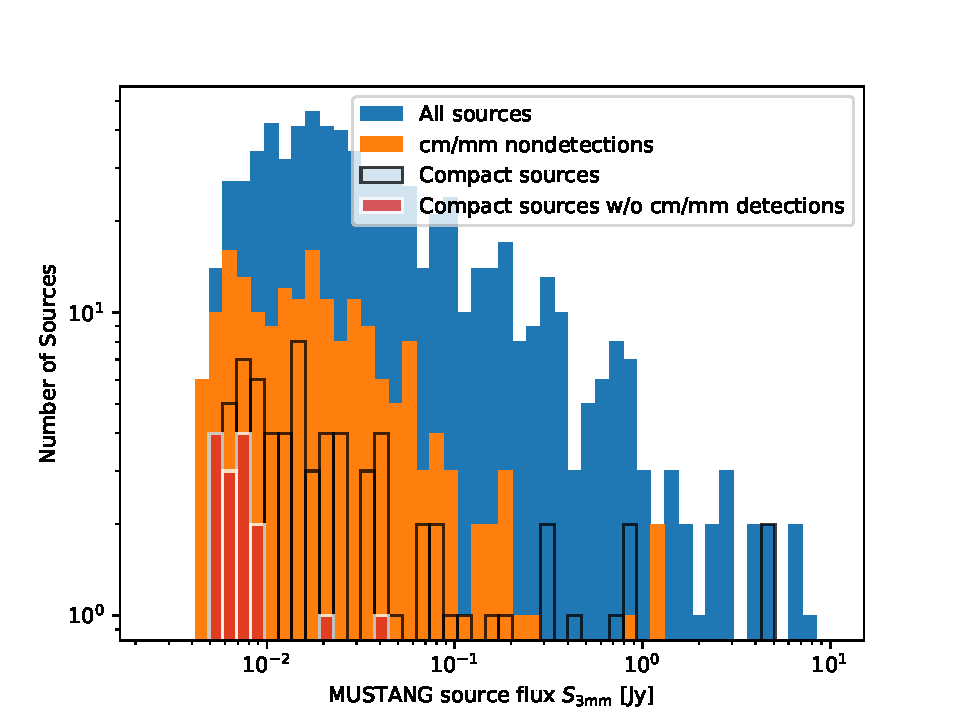
\includegraphics[width=17cm]{figures/full_catalog_histogram.pdf}
    \caption{Histogram of the source catalog.  Blue shows all sources,
    while orange (overlaid on top) shows only those sources that have
    no matches at cm or mm wavelengths in the searched surveys.}
\label{fig:fullcathist}
\end{figure*}


% \todo{Add measurements of known HCHII regions - get those IDs from somewhere.}
% Known HCHIIs are W51 clusters (Ginsburg 2017), W49 objects (De-Pree...),
% G34.26+0.15 (Sewilo), Sgr B2.

% \subsection{W43 catalog}
% We use the W43 region as our test area to examine the cataloging process and
% cross-matching in detail.
% \todo{The old cataloging was performed on the file
% \texttt{GAL\_031\_precon\_2\_arcsec\_pass\_9.fits}.}
% 
% In W43, most (80\%) of the 108 MUSTANG 3mm sources have a corresponding Herschel
% compact source, 49\% have a centimeter association, and only 19\% have a
% Spitzer association.  Visual inspection of the Spitzer maps revealed that there are likely
% infrared sources associated with the majority of the MUSTANG sources, but many
% of these infrared sources are extended objects that were not included in the
% Spitzer GLIMPSE and MIPSGAL catalogs.
% 
% The breakdown of match fraction as a function of flux density is shown in histograms
% in Figure \ref{fig:histogram}.

% \subsubsection{Individual sources}
% While most MUSTANG sources are detected at either millimeter and submillimeter
% wavelengths, representing dust emission, or at centimeter wavelengths,
% representing free-free emission, there are some interesting exceptions.
% 
% Sources with no counterparts at other wavelengths: \\
% G29.955-0.110 (faint) \\
% G29.973-0.285 (Herschel not available) \\
% G30.159-0.466 (faint) \\
% G30.008-0.039 (faint/questionable) \\
% G30.721-0.039 (diffuse counterparts?) \\
% G29.969+0.033 (faint) \\
% G30.364+0.027 (diffuse, faint)\\
% G31.371+0.021 (faint) \\
% 
% 
% Sources with 3mm and cm-and-longer detections, but no IR or FIR or submm detections:\\
% #G30.437-0.206 \\
% G31.150-0.189 \\
% G31.387-0.383 \\
% G30.330+0.090 \\
% G31.440+0.510 (no Herschel 70 \um or 160 \um data available) \\
% 
% 
% Sources with 3mm and Spitzer detections, but no FIR or cm:
% G30.248-0.192 \\
% 
% IRDCs:\\
% G30.400-0.296 \\
% G30.419-0.231 \\
% G30.689+0.032 (faint, questionable)\\
% G30.920+0.091 \\
% G31.382+0.318 \\
% G31.581+0.077 \\



% Source G30.651-0.060 (Figure \ref{fig:sed177}) is detected at 3 mm, but has no counterpart from 160 to 1100 \um or
% at centimeter wavelengths, and only a weak counterpart in the Herschel 70 \um
% data. However, it has a clear and bright detection from 3.6 - 24 \um, indicating
% the presence of a star with surrounding hot dust.  The lack of cm detection suggests
% that hot dust is not part of an ionized region.  It is not clear why 3 mm emission
% is detected.

% Source G29.979+0.021 (Figure \ref{fig:sed22}) is detected at 20 cm, 1.1 and 3 mm, 70 \um,
% and 3.6 - 24 \um.  The lack of far-infrared detections indicates that there is
% no cold dust associated with the source, but the detection at 20 cm and
% nondetection at 6 cm is not consistent.  The most likely explanation for this
% discrepancy is that this source is variable and has a flickering \hii region.

% The brightest source with a Herschel nondetection is G30.711-0.019.  It is in a
% region filled with extended emission at many wavelengths.  The 3 mm emission
% closely matches the 20 cm emission and 70 \um and shorter-wavelength emission,
% but does not match the longer-wavelength millimeter emission, suggesting that
% the 3 mm is dominated by free-free emission.  The millimeter and centimeter
% emission are offset from one another, which is why there was no catalog source
% match; the free-free emission wraps around the dust emission.  This source is
% therefore just a particularly bright patch of diffuse free-free emission.

\subsection{\hchii region identification}
\label{sec:hiireg}
One of the aims of this survey is to identify the youngest high-mass
protostars.  Candidates are those sources with little to no mid-infrared emission
and very compact, optically thick (hypercompact) \hii regions.

Massive stars form in the middle of ultra-dense cores undergoing gravitational
collapse, leading to an accretion rate of order $\dot{M} \sim 10^{-3}$ \msun
\peryr such that a 100 \msun star takes about $10^5$ years to accrete its mass.
As the star contracts onto the main sequence it starts to ionize its
environment to create an \hchii region.  For a sufficiently dense accretion
flow, the Str{\"o}mgren radius of the \hchii regions are bound by the gravity of
the star, with a radius $R_G \sim$50-100 AU
\citep{Keto2002a,Keto2003a,Keto2007a}.  These gravitationally bound \hchii
regions are optically thick at centimeter wavelengths and therefore emit as
blackbodies at wavelengths $\lambda\gtrsim$3~mm, with 
\begin{equation}
    S_\nu=21 \textrm{mJy} \left(\frac{d}{5
    \textrm{kpc}}\right)^{-2} \left(\frac{R}{100 \textrm{AU}}\right)^2 \left(\frac{\nu}{90 \textrm{GHz}}\right)^2
\end{equation}
which is only
0.06 mJy at $\nu=5$ GHz, and therefore below the detection limit of many
existing surveys; they are certainly unremarkable sources at long wavelengths.
\hchii regions can be distinguished from older
ultracompact (\uchii) regions by their  bright 90\,GHz emission and faint emission at 5\,GHz and lower
frequencies.  Sources
with free-free emission that peaks at or just below 3 mm represent the youngest
high-mass YSOs.  The dense cores surrounding these sources will be bright
in the millimeter regime, since they will have high dust column densities and
temperatures.

% Hypercompact \hii regions are defined as $\lesssim0.03$ pc ($\lesssim6000$ AU)
% \hii regions around young stars \citep{Kurtz2005b}.  They have high ionized
% gas density, resulting in a spectrum that remains optically thick to relatively
% high frequency.
We therefore select candidate HC\hii regions
as those fitting either of these criteria:
\begin{enumerate}
    \item $S_{3 \mathrm{mm}} > 1.75 S_{6 \mathrm{cm}}$.  % or $S_{3 \mathrm{mm}} > S_{20 \mathrm{cm}}$.
        This requirement selects free-free sources that have $\tau_{ff}=1$
        at $\lambda = {6 \mathrm{cm}}$.  It corresponds to an emission
        measure ${EM=7\ee{7}~\mathrm{cm}^{-6}~\mathrm{pc}}$.
    \item
        The source is not detected at 6 and 20 cm, is detected at 1.1 mm, and has
        \begin{equation}
            \frac{S_{3 \mathrm{mm}}}{S_{1.1 \mathrm{mm}}} > \left(\frac{\lambda_{3 \mathrm{mm}}}
            {\lambda_{1.1 \mathrm{mm}}}\right)^{-\alpha} = 0.038
        \end{equation}\\
        where $\alpha=3$ is the spectral
        index for optically thin dust with an opacity index $\beta=1$.  This
        requirement selects dust-detected sources in which there is some
        indication of an excess of free-free emission over pure dust emission
        at 3 mm.
        \hchii regions that are optically
        thick up to $\sim3$ mm, those that are extremely compact and dense,
        are below the detection threshold of the centimeter surveys
        \citep[$\approx2.5$ mJy at 6 cm;][]{Giveon2005a,Hoare2012a}.
\end{enumerate}

These criteria provide a small sample of \nhiicand candidate \hchii regions
across the seven target regions.  Only \ncompacthiicand of these candidates
were morphologically compact. This sample consists of known
ultracompact or hypercompact HII region clusters \citep[three are parts of W49A, which contains
12 sources that can be classified as \hchii regions][]{De-Pree1997a},
the \hchii region G34.257+0.153, and the OH/IR star G30.944+0.035.
The ten known \hchii regions in W51 \citep{Ginsburg2016b} were not recovered because
they are blended, in the 9\arcsec \MUSTANG beams, with more diffuse \hii regions.

However, the majority of sources in our catalog do not have
centimeter-wavelength detections and therefore were not
eligible to be selected based on criterion 1 above, and the BGPS 1.1 mm data,
with only 30 \arcsec resolution, could be confused and therefore too bright for
a 3 mm excess to be detected, preventing selection by criterion 2. 

While we would expect some excess above the extrapolated dust emission for
dusty HCHII regions, it is plausible that the excess is not enough to modify
the spectral index to meet our selection criterion 2.  Sources that have
millimeter detections (since they must be surrounded by gas and dust) and not
centimeter detections therefore remain candidate \hchii regions.  This large
sample of \mmdetectionscmnondetections additional candidates, especially the
\mmdetectionscmnondetectionscompact that are compact, are interesting
candidates for future deep centimeter observations.

Several well-known hypercompact \hii regions were excluded from these selection
criteria.  The \hchii regions in W51, including the W51e cluster and W51d2
\citep{Ginsburg2016a}, those in W49 \citep{De-Pree1997a}, and those in Sgr B2
\citep{De-Pree1998a} are confused, residing in the same beams as other
high-mass stars at different evolutionary states.  G34.257+0.153 includes a pair
of \hchii regions but less other surrounding emission, so it did pass our selection
criteria \citep{Sewilo2004a,Avalos2006a}.  MGPS90 is clearly capable of detecting
\hchii regions that are not in dense protoclusters.


\subsection{Constraints on \hchii lifetimes}
To estimate the relative lifetime of the hypercompact and ultracompact phases,
we compare the number of \hchii candidates to the number of detected \uchii
regions from the CORNISH survey \citep{Kalcheva2018a}.  \citet{Wood1989a}
seeded the idea that \uchii lifetimes may be substantially longer than expected
for a freely expanding Strömgren sphere $t_{free expansion} \sim 4\ee{4}$ years,
but the improved sample of \citet{Kalcheva2018a} suggests that the discrepancy
is not so large.  In any case, we adopt a loosely estimated \uchii lifetime somewhere
between $4\ee{4} \mathrm{yr} < t_{\uchii} < 4\ee{5} \mathrm{yr}$.

In the observed regions, the CORNISH survey detected 73 \uchii regions.  Over
the same area, our sample includes \mmdetectionscmnondetectionscompact compact
\MUSTANG sources with no centimeter detections, which are our additional
candidates from \S \ref{sec:hiireg}, and four previously-known \hchii regions.
W51 contains 10 and W49A contains up to 12 additional \hchii region candidates
when viewed at high resolution \citep{De-Pree1997a,Ginsburg2016a}.  The
inferred lifetime of \hchii regions, using a sample size of 12-34 \hchii's in
the \MGPS fields, is therefore $16-46\%$ that of \uchii regions, or $6\ee{3}
\mathrm{yr} < t_{\hchii} < 2\ee{5} \mathrm{yr}$.  A more complete assessment
from the larger survey may more tightly constrain these values.

Furthermore, though, the relatively small number of new candidates (only
\mmdetectionscmnondetectionscompact) compared to the large numbers in compact
regions suggests that \hchii regions
form primarily in, or live longest in, clustered regions.  This high production
of \hchii regions in dense protoclusters can be either because more high-mass stars
form there, indicating an overall higher population, or because the gas density is
higher, allowing the \hii regions to remain in the hypercompact phase for a longer
period before expanding into \uchii or diffuse \hii regions.

% TODO: HCHII lifetime estimates?
% How many UCHII regions exist in our target area?

% G29.977-0.047: SED is dust-only, but there is excess at 3 mm plus a bright 70 \um source.  Could be?
% G30.009-0.273: Compact HII region?  6cm detection, 20cm limit
% G30.099+0.077: Candidate?  24, 70 \um bright.  CH3OH, H2O source
% 
% General conclusion: these are all good candidates, but they may contain mixes of HII regions and MYSOs.
% 
% 
% Source G30.437-0.206 (Figure \ref{fig:sed83}) is detected at 6 cm, 20 cm, and 3
% mm, but has no compact source detections at shorter wavelengths.  There is
% diffuse dust emission from 24 - 1100 \um around this source, indicating that
% dense, cold dust is present.  This source is an excellent candidate for a very
% young hypercompact \hii region.


% \begin{figure*}[htp]
%     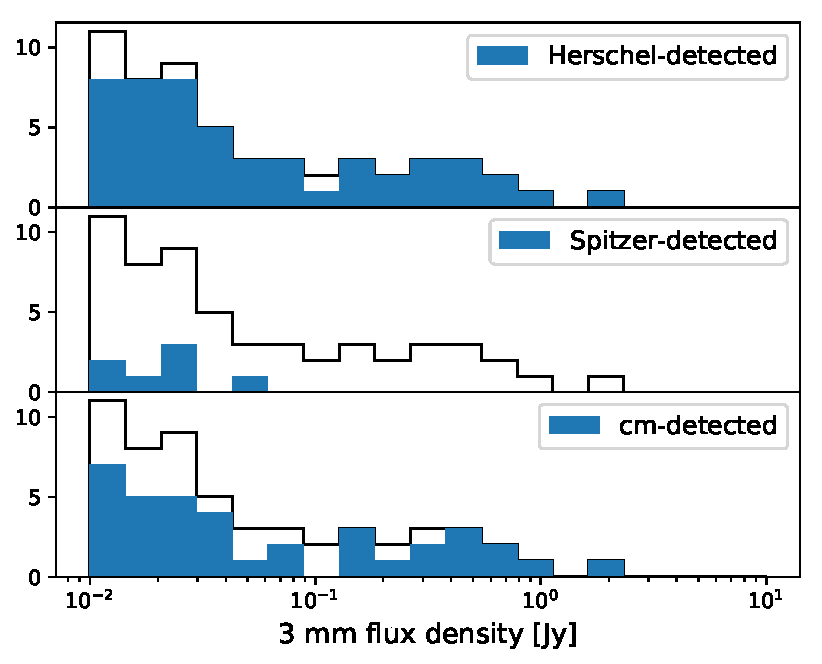
\includegraphics[scale=1]{figures/G31_dend_contour_thr4_minn20_mind1_detection_histograms.pdf}
% \caption{Histograms of the MUSTANG 3mm flux density in the W43 field.  In each
% panel, the colored region shows which sources were detected in one or more of
% the Herschel Hi-Gal (top), Spitzer GLIMPSE or MIPSGAL (middle),
% or MAGPIS 6 or 20 cm or CORNISH 6 cm (bottom) surveys.}
% \label{fig:histogram}
% \end{figure*}


% no longer exists
% \begin{figure*}[htp]
%     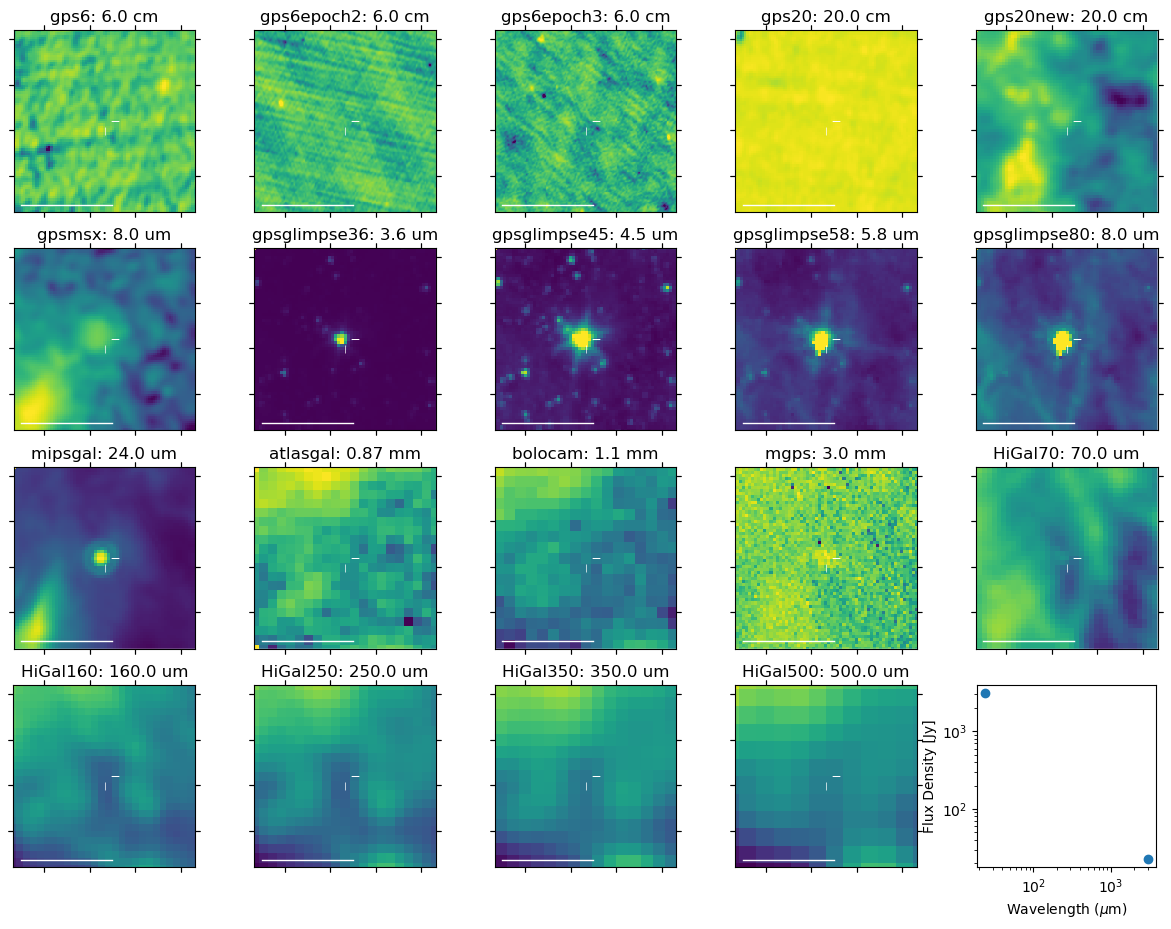
\includegraphics[width=17cm]{figures/SED_plot_G031_177.png}
% \caption{SED plot for Source  G30.651-0.060 from W43.  The panels are labeled with the
% survey and frequency used for the plot.  The data come from the MAGPIS cutout
% server (\url{https://third.ucllnl.org/gps/}) and the Herschel Hi-Gal image
% server (\url{https://tools.ssdc.asi.it/HiGAL.jsp}); references are given in the
% text.  The bottom-right panel shows an SED constructed from the sources matched
% from the catalogs described in Section \ref{sec:catalogmatching}.
% This source is detected only at 3 mm and in the near infrared; it is not clear
% what class of object it is.
% }
% \label{fig:sed177}
% \end{figure*}

% no longer exists
% \begin{figure*}[htp]
%     \includegraphics[width=17cm]{figures/SED_plot_G031_22.png}
% \caption{SED plot for Source G29.979+0.021 from W43.  See Figure \ref{fig:sed177} for a description.
% Because this source is detected at 20 cm and 3 mm, but not at the intermediate 6 cm wavelength,
% it is likely a variable \hii region associated with the central massive star.
% }
% \label{fig:sed22}
% \end{figure*}


% \begin{figure*}[htp]
%     \includegraphics[width=17cm]{figures/SED_plot_G30.437-0.206.png}
%     \caption{SED plot for Source G30.437-0.206 from W43.  The panels are
%     labeled with the survey and frequency used for the plot.  The data come
%     from the MAGPIS cutout server (\url{https://third.ucllnl.org/gps/}) and the
%     Herschel Hi-Gal image server (\url{https://tools.ssdc.asi.it/HiGAL.jsp});
%     references are given in the text.  The bottom-right panel shows an SED
%     constructed from the sources matched from the catalogs described in Section
%     \ref{sec:catalogmatching}.  This source is detected only at 3 mm and longer
%     wavelengths.  It is likely a hypercompact \hii region.}
% \label{fig:sed83}
% \end{figure*}


\begin{figure*}[htp]
\includegraphics[width=17cm]{figures/G01_overview.pdf}
\caption{\MUSTANG image of the G01 field, centered on Sgr B2.
%The green squares show
%sources with millimeter/submillimeter counterparts, blue circles show those
%with centimeter counterparts, purple triangles show sources with \emph{both} millimeter
%and centimeter counterparts, and orange diamonds show those with no millimeter
%or centimeter counterparts.
}
\label{fig:g01overview}
\end{figure*}

\begin{figure*}[htp]
\includegraphics[width=17cm]{figures/G12_overview.pdf}
\caption{\MUSTANG image of the G12 field, including the W33 star-forming region.}
\label{fig:g12overview}
\end{figure*}

\begin{figure*}[htp]
\includegraphics[width=17cm]{figures/G29_overview.pdf}
\caption{\MUSTANG image of the G29 field.}
\label{fig:g29overview}
\end{figure*}


\begin{figure*}[htp]
    \includegraphics[width=17cm]{figures/G31_overview.pdf}
\caption{\MUSTANG image of the G31 field containing W43.
%The overplotted symbols show the locations
%of Herschel-detected sources in cyan crosses, centimeter-detected sources in white x's, centimeter-detected Herschel nondetections as red circles,
%and centimeter and Herschel non-detections in green.
}
\label{fig:w43overview}
\end{figure*}


\begin{figure*}[htp]
\includegraphics[width=17cm]{figures/G34_overview.pdf}
\caption{\MUSTANG image of the G34 field.  Above $b\gtrsim 0\deg$,
horizontal cross-scans have not been obtained; the vertical streak seen
at $\ell=34.25\deg$ is a consequence of these missing data.}
\label{fig:g34overview}
\end{figure*}

\begin{figure*}[htp]
\includegraphics[width=17cm]{figures/G43_overview.pdf}
\caption{\MUSTANG image of the G43 field, which contains the 
W49A star-forming complex (center) and the W49B supernova remnant (just southeast
of center).}
\label{fig:g43overview}
\end{figure*}


\begin{figure*}[htp]
\includegraphics[width=17cm]{figures/G49_overview.pdf}
\caption{\MUSTANG image of the G49 field, which contains the W51 star-forming
complex.}
\label{fig:g49overview}
\end{figure*}

\subsection{Representative SEDs of selected sources}
To put the \MGPS data in context, we show a few examples of SEDs extracted
from the catalogs described in section \ref{sec:catalogmatching} along with
cutout images extracted from the same surveys.  The selected SEDs are of a
planetary nebula (Fig. \ref{fig:g29pn}), which exhibits emission at all
wavelengths, an OH/IR star (Fig. \ref{fig:g31ohir}) that is infrared- and
millimeter-bright but not detected at centimeter wavelengths, a high-mass
YSO that is a candidate \hchii region with no centimeter detection (Fig.
\ref{fig:g12hiicand}), and a source containing a known pair of \hchii regions
(Fig.  \ref{fig:g34hchii}).  These SEDs highlight the important role of \MGPS
data in bridging the gap between the millimeter and centimeter regimes.

%\todo{In this section, we'll show SEDs of a few selected sources (HCHII region, UCHII region,
%dust-only source, OH/IR star, whatever) along with the cutout mosaic.}
% candidates: G11.943-0.156: dust-only, detected at infrared but not cm.  Bright mm.  BGPS spatially offset
% G11.945-0.036: extended HII region (why no 20cm counterpart in catalog?)
% G11.971+0.192: likely extragalactic, possible radio jet
% G12.116+0.077: DHII deeply embedded HII region
% G12.153-0.331: DHII maybe same as above?  less clear case
% G12.154+0.413: very compact, free-free only (flat spectrum) source.  No detections <3mm
% G12.199-0.034: very clean SED, with detections at every wavelength.  Compact.  Star?  RMS class is HII region
% G12.208-0.102: dense HII region, UCHII but not HCHII.  Full SED
% G12.332-0.180: DHII ?
% G12.889+0.490: deeply embedded, no free-free: candidate HCHII?
% G12.908-0.260: star?
% G29.578-0.267: full SED.  Star?  Coordinate offset evident; check if this one is fixed w/re-cataloging.  CONFIRMED planetary nebula
%  CLEAR pointing offset in G29 means cataloging needs to be redone [I did that]
% G30.530+0.132: 


\begin{figure*}[htp]
\includegraphics[width=17cm]{figures/SED_plot_G29_G29.578-0.268.pdf}
\caption{SED of source G29.578-0.268, a planetary nebula.  The individual panels show cutouts from 
various surveys hosted on the MAGPIS cutout service
(\url{https://third.ucllnl.org/gps/}) and the Herschel Hi-Gal cutout service
(\url{https://tools.ssdc.asi.it/HiGAL.jsp}); individual survey references are in Section \ref{sec:catalogmatching}.
The white bar in the lower-left is a 1\arcmin\ scalebar.
Short wavelengths ($<24$ \um) are not included in the SED, the rest are included in the cross-matched catalog.
}
\label{fig:g29pn}
\end{figure*}


\begin{figure*}[htp]
\includegraphics[width=17cm]{figures/SED_plot_G12_G12.026-0.031.pdf}
\caption{SED of source G12.026-0.031, a candidate \hchii region and likely high-mass YSO identified in the RMS
survey \citep{Lumsden2013a}.  This compact source failed the criteria in Section \ref{sec:hiireg},
indicating that no clear excess of free-free emission is detected at 3 mm, and suggesting that if an \hchii region is
present, it is faint.  Such objects are of particular interest because they constitute the most compact and likely youngest
forming high-mass stars.}
\label{fig:g12hiicand}
\end{figure*}



\begin{figure*}[htp]
\includegraphics[width=17cm]{figures/SED_plot_G31_G30.944+0.035.pdf}
\caption{SED of source G30.944+0.035, an OH/IR star.  The dusty SED with no
detected radio emission made this source a candidate hypercompact HII region
based on the criteria in Section \ref{sec:hiireg}, though it only barely passed
the second criterion.}
\label{fig:g31ohir}
\end{figure*}

\begin{figure*}[htp]
\includegraphics[width=17cm]{figures/SED_plot_G34_G34.257+0.153.pdf}
\caption{SED of source G34.257+0.153, which contains several \hchii regions
within the MGPS90 beam.  The source passed the selection criteria in Section
\ref{sec:hiireg}, confirming that these are useful criteria for identifying
relatively isolated \hchii regions. The intermediate Herschel wavelengths (160,
250, 350 \um) appear as upper limits because the HiGal catalogs broke this
source into several, none of which match the MGPS90 centroid to within
10\arcsec.  The asymmetry in the \MGPS image is caused by the missing
scans noted in Figure \ref{fig:g34overview}.}
\label{fig:g34hchii}
\end{figure*}


\section{Diffuse Emission: Free-free separation}
\label{sec:freefree}
As stated in the introduction, the MGPS90 data have contributions from thermal
free-free, thermal dust continuum, and nonthermal synchrotron emission.  We
describe here our decomposition of the MGPS90 data into free-free and dust
emission; the non-thermal emission was not separated from the free-free
emission.


We use the ATLASGAL 870\,$\mu$m data \citep{Schuller2009a} to estimate the dust
contribution since at 870\,$\mu$m essentially all emission is from dust.  We
estimate the 90\,GHz flux density from dust by scaling the ATLASGAL data
assuming a dust emissivity index $\beta=1.5$.  Using this value of $\beta$, the
ATLASGAL 870\,$\mu$m and MGPS90 data flux densities are related via $S_{\rm
90GHz} \simeq 0.013 S_{\rm 870\mu m}$ (cf. Equation~\ref{eq:dust}).  We
subtract the scaled ATLASGAL data from an appropriately smoothed version of the
MGPS90 map to obtain an estimated free-free map.  We perform this subtraction
on the feathered MGPS90 and Planck data (Section~\ref{sec:feather}).

Similarly, we use 20 cm maps to estimate the dust contribution by subtracting
a scaled 20 cm map from the MGPS90 data.
%We compare the resultant ff+s maps with VLA images made at 20\,cm to gain insight into
%the relative contributions from free-free and synchrotron emission.  
%Sources with negative spectral indices will appear brighter at 20\,cm than at 90\,GHz.
For most fields, we use 20\,cm MAGPIS data \citep{Helfand2006a}, which has an
angular resolution of $\sim\!6\arcsec$ and a point source sensitivity of
$1-2$\,mJy.  MAGPIS does not cover the Galactic center or 
$\ell>48^\circ$, and so we use other data in these zones. In the Galactic
center, we use the multi-configuration 20 cm map from \citet[][resolution
$\sim30\arcsec$]{Yusef-Zadeh2004a}, and in the W51 field we use the
multi-configuration map from \citet[][resolution $\lesssim1\arcsec$]{Mehringer1994a}.
We scale the 20 cm to 90 GHz assuming the 20 cm consists exclusively of optically
thin free-free emission  following a power law $S_{\nu}
\propto \nu^{-0.12}$ \citep{Wilson2009a}.  If the power law has a more negative
spectral index, 
%when the scaled 20\,cm data is subtracted from the 3\,mm MGPS data,
the resultant ``3\,mm Dust'' image will have negative values; if it is
more positive, the resultant image will have positive values.  The observed
fields were selected
based on their rich ongoing star formation activity, so this approximation is
reasonable, but there are several cases where additional emission mechanisms
(e.g., synchrotron)
must be active.
%(which is incorrect; these maps contain both synchrotron
%emission and optically thick free-free emission)

We show the results of the decomposition for one example field in
Figure~\ref{fig:arches_freefree}; the rest of the MGPS90 fields are in the
Appendix.  Figure~\ref{fig:arches_freefree} contains panels of the MGPS90 data,
the contribution to the MGPS90 data from thermal dust estimated from ATLASGAL
subtraction, the contribution to the MGPS90 data from ff+s, 20\,cm data, and
the contribution to the MGPS90 data from thermal dust estimated from 20\,cm
subtraction.

%The ratio
%map  gives an indication of the ff+s spectral index, and can allow one to
%separate thermal and nonthermal emission.}  We expect that the ratio $S_{\rm
%90GHz}/S_{\rm 20cm} \simeq 0.25$ for optically-thin free-free emission and is
%less than this value for synchrotron emission.

The example in Figure \ref{fig:arches_freefree} shows good agreement between the
two dust estimates and between the free-free estimates, and the differences
highlight some of the incorrect assumptions in the above analysis.  The excess
diffuse emission in the rightmost panel (MGPS90 - VLA) is most likely caused by
the VLA's failure to recover large angular scales.  The missing emission on the
right side of that map is caused by the excess synchrotron emission in the Sgr
A region, which is not accounted for in our simple free-free model.  Both dust
maps do well at recovering emission from the massive G0.253+0.015 cloud (the bean-shaped
feature in the upper left) and the southern dust ridge (the prominent dust feature
just below the center of the map).

The W43 region is substantially more dust-dominated than the Galactic Center
(Figure \ref{fig:w43freefree}).  The dusty features, however, are all closely
aligned with free-free features, so it is difficult to disentangle them by eye
in the MGPS90 image.  The MGPS90 - 20 cm image is negative in the 20
cm-dominated regions, likely indicating that there is substantial nonthermal
emission in these HII regions.  While there are no known supernovae in the region, the population
of OB and Wolf-Rayet stars powering the expanding HII region may also
drive strong shocks into the surrounding medium \citep[e.g.][]{Bally2010a}, leading to nonthermal emission.
The presence of such nonthermal emission indicates that electrons must be
accelerated to relativistic velocities in the HII region, which has recently
been shown to be possible in HII region expansion fronts
\citep{Padovani2019a}.

The W49B supernova remnant in the G43 field stands out as a bright nonthermal
source.  No other supernova remnants in the surveyed area are as bright at 3\,mm (see
Figure~\ref{fig:g43overview}). \citet{Sun2011a} found that the spectral energy
distribution of W49B is well-fit by a single power law from 200\,MHz to 30\,GHz
with index $\alpha=-0.46\pm0.01$.  They found that the 5\,GHz integrated flux density is
$19.10\pm0.98$\,Jy, and the 90\,GHz integrated flux density should be 5.1\,Jy.
%(90/5)^(-0.46)*19.1 . 
Integrating over W9B, we find a flux density of 5.2\,Jy, indicating that most of
the associated emission is nonthermal. 
% note to Loren: the alpha=4.6 scaling results in the bright edges going to ~zero,
% but the center ends up too low, suggesting that the center (the faint bit) is
% consistent w/-0.12 but the edges are ~-0.46.  It's beyond the scope of this
% paper to go into that level of detailed analysis, though

\begin{table*}[htp]
\centering
%\begin{minipage}{130mm}
\caption{Free-free and Dust Emission Fractions}
\begin{tabular}{llll}
    \label{tab:freefree}
Field Name   & Center (Galactic) & Field Size & Dust Fraction ($\beta=1.5$) \\
             & degrees           & arcminutes &                             \\
\hline
\hline
Arches     & 0.140 -0.054                        & 12.60 &        0.08 \\
Sgr\,B2    & 0.657 -0.041                        & 12.80 &        0.13 \\
W33        & 12.805 -0.206                       &  3.72 &        0.11 \\
G29        & 29.927 -0.041                       &  5.87 &        0.11 \\
W43        & 30.757 -0.045                       &  7.24 &        0.10 \\
G34        & 34.257 0.148                        &  2.80 &        0.21 \\
W49a       & 43.171 -0.006                       &  4.38 &        0.13 \\
W49b       & 43.268 -0.186                       &  3.53 &        0.04 \\
W51a       & 49.461 -0.368                       &  8.75 &        0.14 \\
W51b       & 49.080 -0.338                       & 11.30 &        0.07 \\

\hline
\hline
\end{tabular}
% \par this is a caption.
\end{table*}

We directly quantify the dust contribution to the 3 mm intensity in the
targeted brightest fields.  Each field includes one or more prominent extended
structures that were the focus for these pilot observations.  For each of these
structures, we extracted an area that encompasses the bulk of the 3 mm emission
and measured the fraction of that emission that is explained by optically-thin
dust, which is the sum of the positive values from the scaled ATLASGAL data
explained above divided by the sum of the 3 mm emission.  The results are reported
in Table \ref{tab:freefree}.  Because we have assumed $\beta=1.5$, and typical
dust $\beta$ values for the ISM are $\sim1.5-2$ \citep[e.g.,][]{Ossenkopf1994a},
these can be treated as upper limits on the dust contribution.

In the regions of interest, the dust contribution at 3 mm is limited to
$\lesssim20\%$ on the several arcminute scales probed.  Regions with substantial
synchrotron contributions from supernova remnants (W49b, W51b) or other mechanisms
(the Arches) have an even lower contribution from dust, $<10\%$.  In short, the 
integrated diffuse emission detected in MGPS90 is dominated by emission from hot gas rather
than from cold molecular gas.  We are, however, unable to determine whether the \emph{area}
of the survey is dominated by hot or cold gas, as the large angular scale filtering of the
interferometric data sets prevents such an assessment; it remains possible that the area
(and volume) of the surveyed regions is dominated by cold dust emission, while the received
flux is clearly dominated by hot gas.




%However,
%despite this clear oversubtraction, the difference image shows an exquisite
%high-resolution view of the compact dust-dominated features.

%To get a better sense of what is detected, we do the stuff in freefree\_dust\_separation.py

\begin{figure*}[htp]
    \includegraphics[width=17cm]{figures/G01_arches_5panel.pdf}
    \caption{Decomposition of the MGPS90 data in the Sgr B2 field centered on the Arches region. 
    All images are displayed on the same intensity scale.  In the G01 field,
    the 20 cm data have 30\arcsec resolution, so the MGPS90 data have been smoothed to match
    the resolution of the other images.
    (a; 870 \um scaled) ATLASGAL 870 \um scaled to 3 mm
    (b; 3 mm free-free) smoothed MGPS90 - scaled ATLASGAL
    (c; 3 mm) MGPS90 
    (d; 3 mm Dust) smoothed MGPS90 - scaled VLA 20 cm continuum.
    (e; 20 cm scaled) VLA 20 cm continuum scaled to 3 mm
}
\label{fig:arches_freefree}
\end{figure*}

\begin{figure*}[htp]
    \includegraphics[width=17cm]{figures/G31_w43_5panel.pdf}
    \caption{Decomposition of the MGPS90 data in the G31 field centered on W43.
    See Figure \ref{fig:arches_freefree} for a description of the panels.
    In G31, the 20 cm data have $\sim5$ \arcsec resolution, so they are
    smoothed to match the MGPS90 data to create panels (d) and (e), while the
    MGPS90 data are smoothed to match the ATLASGAL data to create panel (b).
}
\label{fig:w43freefree}
\end{figure*}





\section{Conclusions}
We have presented the pilot data for the MUSTANG 90 GHz Galactic Plane
Survey, MGPS90.  When complete, this survey
will cover most of the northern Galactic plane within $b<0.5$.
These initial data cover several high-mass star cluster
forming regions.  All imaged regions are dominated by free-free and synchrotron
emission at 3 mm.  

We cataloged emission in the images, identifying \nsources compact sources using the
\texttt{dendrogram} algorithm, of which \ncompacthiicand are verified \hchii
regions, and another \mmdetectionscmnondetectionscompact are plausible
candidates.  

\acknowledgements
\MUSTANG is funded by the NSF award number 1615604 and by the Mt.\ Cuba
Astronomical Foundation. The National Radio Astronomy Observatory is a facility
of the National Science Foundation operated under cooperative agreement by
Associated Universities, Inc.



\appendix

\section{Additional free-free / dust decomposition maps}
In this appendix, we show cutout images focused on a selection of bright extended emission regions
and the associated free-free decomposition described in Section \ref{sec:freefree}

\begin{figure*}[htp]
    \includegraphics[width=17cm]{figures/G01_sgrb2_5panel.pdf}
    \caption{Decomposition of the MGPS90 data in the G01 field centered on Sgr B2.
    See Figure \ref{fig:arches_freefree}.
    The differences in the ATLASGAL- and 20 cm-based dust decomposition highlight the
    different angular scales recovered by those data sets.
}
\label{fig:sgrb2freefree}
\end{figure*}

\begin{figure*}[htp]
    \includegraphics[width=17cm]{figures/G12_w33_5panel.pdf}
    \caption{Decomposition of the MGPS90 data in the G12 field centered on W33.
    See Figure \ref{fig:arches_freefree} for a description of the panels.
    The diffuse free-free emission is well-removed by subtracting the 20 cm data,
    but the compact point source appears much brighter in the 3 mm-derived map;
    this difference is likely because free-free emission is present but optically
    thick at 20 cm, resulting in an underestimate of the free-free contribution 
    at 3 mm.
}
\label{fig:w33freefree}
\end{figure*}

\begin{figure*}[htp]
    \includegraphics[width=17cm]{figures/G29_g29_5panel.pdf}
    \caption{Decomposition of the MGPS90 data in the G29 field.
    See Figure \ref{fig:arches_freefree} for a description of the panels.
    Some of the compact structures exhibit strong excesses at 20 cm.
}
\label{fig:g29freefree}
\end{figure*}

\begin{figure*}[htp]
    \includegraphics[width=17cm]{figures/G34_g34_5panel.pdf}
    \caption{Decomposition of the MGPS90 data in the G34 field centered on G34.26+0.15.
    See Figure \ref{fig:arches_freefree} for a description of the panels.
    The vertical streak is an artifact as mentioned in Figure \ref{fig:g34overview}.
}
\label{fig:g34freefree}
\end{figure*}


\begin{figure*}[htp]
    \includegraphics[width=17cm]{figures/G43_w49a_5panel.pdf}
    \caption{Decomposition of the MGPS90 data in the G43 field centered on W49A.
    See Figure \ref{fig:arches_freefree} for a description of the panels.
    As in Figure \ref{fig:g29freefree}, several compact structures appear to have
    excess 20 cm emission.  However, other structures exhibit free-free
    emission that is optically thick at 20 cm and is therefore under-subtracted
    at 3 mm in panel (d); see also Figure \ref{fig:w51mainfreefree}.
}
\label{fig:w49afreefree}
\end{figure*}

\begin{figure*}[htp]
    \includegraphics[width=17cm]{figures/G43_w49b_5panel.pdf}
    \caption{Decomposition of the MGPS90 data in the G43 field centered on W49B.
    See Figure \ref{fig:arches_freefree} for a description of the panels.
    W49B is a supernova remnant completely dominated by synchrotron emission.
    Panel (b) therefore shows synchrotron, not free-free, emission.
}
\label{fig:w49bfreefree}
\end{figure*}

\begin{figure*}[htp]
    \includegraphics[width=17cm]{figures/G49_w51main_5panel.pdf}
    \caption{Decomposition of the MGPS90 data in the G49 field centered on W51 Main.
    See Figure \ref{fig:arches_freefree} for a description of the panels.
    There is a mix of under- and over-subtracted emission in the dust map in panel (d);
    the arc shape in the center is purely free-free emission \citep{Ginsburg2016a,Ginsburg2017a}, but
    it is optically thick at 20 cm.
}
\label{fig:w51mainfreefree}
\end{figure*}




\bibliographystyle{aasjournal}
\bibliography{bibdesk}
\end{document}
